% GraphML (HP3) final report — 25C15053
% Build: xelatex 25C15053.tex (twice)
\documentclass[conference,a4paper]{IEEEtran}
\IEEEoverridecommandlockouts
\usepackage{fontspec}
\setmainfont{Times New Roman}
\usepackage{amsmath,amssymb}
\usepackage{pdfpages}
\usepackage{booktabs,multirow,array}
\usepackage{graphicx}
\usepackage{xcolor}
\usepackage{tikz}
\usetikzlibrary{arrows.meta,positioning,backgrounds}
\usepackage{pgfplots}
\usepackage[hidelinks]{hyperref}
\usepackage{url}
\usepackage{cite}
\usepackage{microtype}
\usepackage{balance}  % equal-height columns on the last page

\setsansfont{texgyreheros}[Extension=.otf,UprightFont=*-regular,BoldFont=*-bold,ItalicFont=*-italic,BoldItalicFont=*-bolditalic]
\usepackage{fontawesome5}
\usetikzlibrary{calc,shapes.geometric}
% Figures live in figures/*.tex (one file per figure, with its data source); shared palette
% and chart style in figures/style.tex, following the paper-figures skill.
% Shared colours and chart styles for the report figures (loaded in the preamble).
% Palette from the paper-figures skill (PaperBanana style guide): pastel zones at ~13%,
% cool tones for frozen models, warm tones for what the paper adds, red only for failures.
\definecolor{gz}{HTML}{9CA3AF}\definecolor{bz}{HTML}{6FA8F5}\definecolor{yz}{HTML}{F2C14E}
\definecolor{pk}{HTML}{F4A7A7}\definecolor{dr}{HTML}{8B2E2E}\definecolor{db}{HTML}{1F4E8C}
\definecolor{peach}{HTML}{FBE3D2}\definecolor{gold}{HTML}{B8860B}
\definecolor{pass}{HTML}{9FD39A}\definecolor{fail}{HTML}{E06666}
\definecolor{tl}{HTML}{9ED9D2}\definecolor{dt}{HTML}{1D5C57}
% series: APKGC and the runs we highlight (warm, key result) versus NativE / baselines (cool)
\colorlet{apk}{dr}
\colorlet{nat}{db}

% Charts: white background, dotted grid, sans labels, legend in one row below.
\pgfplotsset{compat=1.17,
  paperchart/.style={
    axis lines*=left, axis line style={black!60, line width=0.6pt},
    tick style={black!60}, major tick length=2pt,
    grid style={black!30, dotted, line width=0.5pt},
    every tick label/.append style={font=\sffamily\scriptsize},
    label style={font=\sffamily\scriptsize},
    title style={font=\sffamily\scriptsize\bfseries},
    legend style={font=\sffamily\scriptsize, draw=none, fill=none, legend columns=-1,
      /tikz/every even column/.append style={column sep=7pt},
      at={(0.5,-0.32)}, anchor=north},
    legend cell align=left,
    /pgf/number format/assume math mode=true,
    every node near coord/.append style={font=\sffamily\scriptsize}}}

\newcommand{\wb}[2]{\href{https://wandb.ai/nhantrnh-graphml/#1}{{\normalfont\ttfamily #2}}}
\newcommand{\repo}{\url{https://github.com/nhantrnh/GraphML}}
\newcommand{\verdict}[1]{\textbf{#1}}

\begin{document}


\includepdf[pages=1]{cover.pdf}
\setcounter{page}{1}

\title{APKGC and ImparTail}
\author{\IEEEauthorblockN{Trương Thành Nhân}
\IEEEauthorblockA{Student ID 25C15053, Faculty of Information Technology\\
University of Science, VNU-HCM}}
\maketitle

\begin{abstract}
We reproduce two graph learning papers and test each of their claims with the released
code. APKGC adds adaptive noise sampling and an attention penalty to multi-modal knowledge
graph completion. Its headline MRR on MKG-W is approximately reproduced (0.3691 against
0.374 with the paper's configuration; 0.3605 $\pm$ 0.0009 over three seeds with the
released run script), but the claimed sources of the gain are not: the released attention
penalty never fires in 300 measured forward passes and four implementations of it give no
gain, the learnable noise level is driven to about 0 during training, a retrained NativE
baseline scores higher than APKGC under one shared protocol, and a test-time corruption
study shows APKGC to be less robust than NativE in all 30 conditions, collapsing from 0.36
to 0.06 MRR when entity descriptions are swapped. ImparTail masks labels in the loss to
reduce long-tail bias in video scene graph generation. Its STTran baseline is reproduced
within 0.74 mean Recall points on average, but the released code turns masked labels into
negative labels instead of removing them as Eq.~(5) states, and the paper's mask algorithm,
taken literally, would mask the rarest classes entirely. Following Eq.~(5) raises
Recall@50 by 9.4 and 11.4 points under two of three constraints in one unseeded run per
variant, but the run-to-run noise in that setting is of the same order.
\end{abstract}

\begin{IEEEkeywords}
multi-modal knowledge graph, knowledge graph completion, spatio-temporal scene graph, long-tail distribution, reproducibility
\end{IEEEkeywords}

% ═══════════════════════════════ INTRODUCTION ═══════════════════════════════
\section{Introduction}
The two papers in this report come from different areas of graph learning but invite
the same question: \emph{do the published results come from the components the paper
proposes?} APKGC~\cite{apkgc} completes multi-modal knowledge graphs, predicting missing
edges when each entity also has an image and a text description. ImparTail~\cite{impartail}
generates scene graphs from video, where nodes are objects and edges are their relations
over time, with a focus on rare relations.

For each paper we list its claims, rerun the released code, and design one experiment per
claim. Fig.~\ref{fig:verdicts} summarises the outcome; the rest of the report follows the
same order. Every statement about source code has the form ``the released code does X'':
we observe the code, not the authors' experimental process. Equation numbers follow the
paper under discussion.

The code and instructions for rerunning the experiments are at \repo, and the runs are
logged in two public W\&B projects,
\href{https://wandb.ai/nhantrnh-graphml/apkgc-repro}{\nolinkurl{apkgc-repro}} and
\href{https://wandb.ai/nhantrnh-graphml/impartail-repro}{\nolinkurl{impartail-repro}}. Every table and figure that
reports our runs ends its caption with the IDs of the corresponding runs on Weights \&
Biases (W\&B); each ID links to \nolinkurl{wandb.ai/nhantrnh-graphml/<project>/runs/<ID>}.
The runs were built from result files saved after running on Kaggle.

\begin{figure*}[!t]
\centering
\resizebox{\textwidth}{!}{% Figure (full width): the claims of both papers and our verdict on each (Introduction).
% Message: the headline numbers hold approximately, but most mechanism claims of APKGC do not;
% ImparTail's baseline reproduces and its released mask differs from the paper.
% source: Sections IV and VIII of this report (numbers checked by qa/verify_numbers.py).
% Verdict cells use the pass/fail colours: pass = reproduced, fail = not reproduced or not
% supported, yellow = partial or code differs, grey = inconclusive or not tested.
\begin{tikzpicture}[x=1cm, y=1cm, font=\sffamily\scriptsize,
  zone/.style={rounded corners=12pt, fill=#1!13, draw=#1!75!black, line width=1pt, dash pattern=on 4.5pt off 3pt},
  claim/.style={anchor=north west, align=left, text width=#1, inner sep=0pt, font=\sffamily\scriptsize\bfseries, execute at begin node={\hyphenpenalty=10000\exhyphenpenalty=10000}},
  ev/.style={anchor=north west, align=left, text width=#1, inner sep=0pt, font=\sffamily\scriptsize, execute at begin node={\hyphenpenalty=10000\exhyphenpenalty=10000}},
  cell/.style={draw=black, line width=0.8pt, fill=#1, minimum width=1.9cm, minimum height=0.6cm,
               font=\sffamily\scriptsize\bfseries, inner sep=1pt, align=center, anchor=north},
  sec/.style={font=\sffamily\scriptsize, text=black!55, anchor=north, inner sep=1.5pt},
  ztl/.style={font=\sffamily\small\bfseries, anchor=north west, inner sep=0pt},
  hdr/.style={font=\sffamily\scriptsize\itshape, text=black!55, anchor=west, inner sep=0pt}]
% ---------------- APKGC ----------------
\draw[zone=bz] (0,0.55) rectangle (10.3,-5.55);
\node[ztl] at (0.3,0.35) {APKGC (AAAI 2025)};
\node[hdr] at (0.3,-0.25) {claim of the paper}; \node[hdr] at (4.0,-0.25) {our evidence};
\node[hdr] at (8.25,-0.25) {verdict};
\foreach \y/\c/\e/\v/\f/\s in {
  -0.55/{Headline MRR 0.374 on MKG-W}/{0.3691 with the paper's configuration; 0.3605 ± 0.0009 with the run script}/{Approximately}/{yz!70}/{Sec.~IV-A},
  -1.55/{APKGC beats NativE}/{a retrained NativE scores higher under both checkpoint rules}/{Not reproduced}/{fail!60}/{Sec.~IV-A},
  -2.55/{Attention penalty adds 0.014 MRR}/{fires in 0 of 300 passes; four implementations give no gain}/{Not reproduced}/{fail!60}/{Sec.~IV-B},
  -3.55/{Adaptive noise adds 0.016 MRR}/{$\theta_r$ learned to −0.0004; removing noise gives +0.0026 (one seed)}/{Inconclusive}/{gz!45}/{Sec.~IV-C},
  -4.55/{Noise makes the model robust}/{below NativE in all 30 corruptions; 0.0598 with swapped text}/{Not supported}/{fail!60}/{Sec.~IV-D}} {
  \node[claim=3.5cm] at (0.3,\y) {\c};
  \node[ev=3.9cm] at (4.0,\y) {\e};
  \node[cell=\f] (v) at (9.2,\y+0.08) {\v};
  \node[sec] at (v.south) {\s};
  \ifdim\y pt>-4.5pt \draw[black!20, line width=0.4pt] (0.3,\y-0.88) -- (10.0,\y-0.88); \fi}
% ---------------- ImparTail ----------------
\draw[zone=yz] (10.6,0.55) rectangle (18.6,-5.55);
\node[ztl] at (10.9,0.35) {ImparTail (CVPR 2025)};
\node[hdr] at (10.9,-0.25) {claim of the paper}; \node[hdr] at (13.45,-0.25) {our evidence};
\node[hdr] at (16.45,-0.25) {verdict};
\foreach \y/\c/\e/\v/\f/\s in {
  -0.55/{STTran baseline mean Recall}/{nine values within 0.74 points on average}/{Reproduced}/{pass!80}/{Sec.~VIII-A},
  -1.75/{Masked labels leave the loss (Eq.~(5))}/{the code turns them into negatives; Eq.~(5) gains (R@50 +9.4, +11.4) are within run noise}/{Code differs}/{yz!70}/{Sec.~VIII-B},
  -3.15/{STTran mR@20 +51.9\%}/{needs full training of both models over several seeds}/{Not tested}/{gz!45}/{}} {
  \node[claim=2.3cm] at (10.9,\y) {\c};
  \node[ev=2.75cm] at (13.45,\y) {\e};
  \node[cell=\f, minimum width=1.75cm] (v) at (17.35,\y+0.08) {\v};
  \node[sec] at (v.south) {\s};}
\draw[black!20, line width=0.4pt] (10.9,-1.5) -- (18.3,-1.5);
\draw[black!20, line width=0.4pt] (10.9,-2.9) -- (18.3,-2.9);
% legend in one row below both panels
\begin{scope}[shift={(2.2,-6.0)}]
\foreach \x/\f/\t in {0/pass!80/{reproduced}, 3.0/yz!70/{approximately, or code differs}, 7.7/fail!60/{not reproduced, or not supported}, 12.4/gz!45/{inconclusive, or not tested}} {
  \fill[\f, draw=black, line width=0.6pt] (\x,-0.1) rectangle ++(0.32,0.2);
  \node[anchor=west, inner sep=0pt, font=\sffamily\scriptsize] at (\x+0.45,0) {\t};}
\end{scope}
\end{tikzpicture}
}
\caption{The claims of both papers and our verdict on each, with the section that holds the evidence.}
\label{fig:verdicts}
\end{figure*}

% ═══════════════════════════════ PART I ═══════════════════════════════
\section*{PART I: APKGC}

\section{Background and Method}
\subsection{Task and metrics}
A knowledge graph stores facts as triples $(h,r,t)$: head entity, relation, tail entity.
Knowledge graph completion (KGC) answers queries $(h,r,?)$ or $(?,r,t)$ by scoring every
candidate entity and ranking them. In a multi-modal graph each entity also has an image
and a description, which can separate candidates that the graph structure alone cannot.
We report MRR, the mean reciprocal rank of the correct answer, and Hits@$K$, the fraction
of queries whose answer is ranked in the top $K$:
\begin{equation*}
\mathrm{MRR}=\frac{1}{|Q|}\sum_{q\in Q}\frac{1}{\mathrm{rank}_q},\quad
\mathrm{H@}K=\frac{1}{|Q|}\sum_{q\in Q}\mathbf{1}[\mathrm{rank}_q\le K],
\end{equation*}
both in the \emph{filtered} setting, where the other true answers of a query are removed
from its ranking.

The paper places itself among four directions of earlier work: modality fusion (e.g.\
IKRL~\cite{ikrl}, OTKGE~\cite{otkge}, NativE~\cite{native}), better negative sampling
(MMRNS~\cite{mkgw}, MANS~\cite{mans}, AdaMF~\cite{adamf}), combining per-modality decisions
(IMF~\cite{imf}), and noise (SnAg~\cite{snag}). It names two limitations of that work. First, real
multi-modal data is noisy, yet earlier methods try to remove noise rather than become
robust to it. Second, the language models that encode text show \emph{attention
over-trust}, a term from OPERA~\cite{opera}: they put attention on tokens with little
meaning, such as punctuation.

\begin{figure*}[t]
\centering
\resizebox{\textwidth}{!}{% Figure (full width): the APKGC architecture as described in the paper, redrawn (Section II-B).
% Message: noise is added to the raw text vector and image patches before tokenisation (a); the
% penalty acts on attention scores before the BERT/BEiT encoders (b); scoring reuses RotatE (c).
% Equation numbers refer to the APKGC paper. In the released code the encoders instead run once
% beforehand and are frozen (see figures/flow.tex). Schematic, no values.
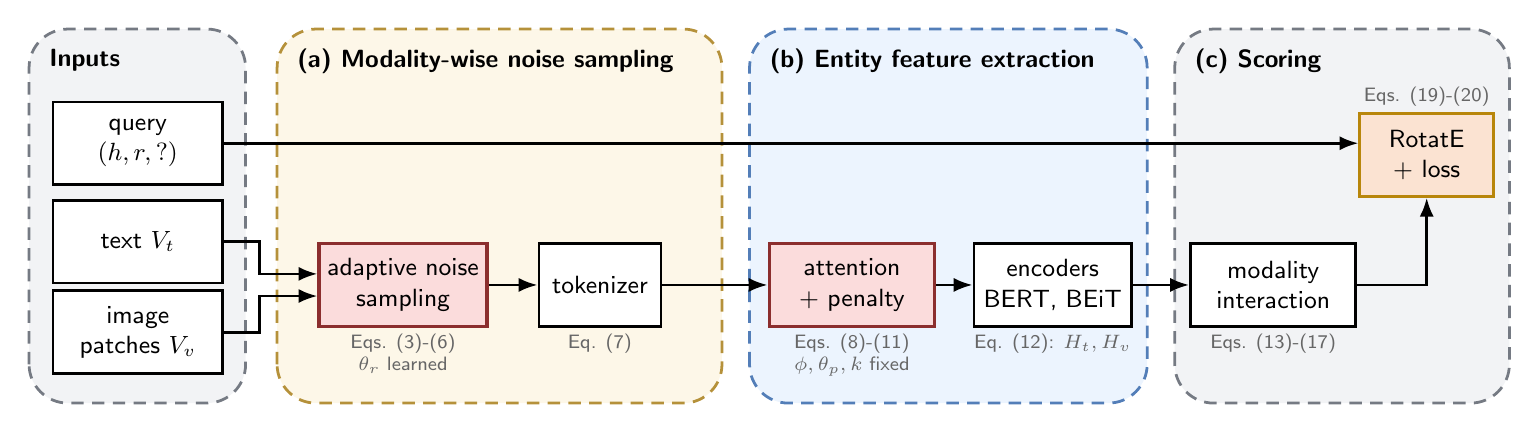
\begin{tikzpicture}[x=1cm, y=1cm, font=\sffamily\small,
  box/.style={draw=black, line width=1pt, fill=white, align=center, font=\sffamily\small, inner sep=3pt,
              minimum height=1.05cm},
  added/.style={box, fill=pk!40, draw=dr, line width=1.2pt},
  outbox/.style={box, fill=peach, draw=gold},
  zone/.style={rounded corners=14pt, fill=#1!13, draw=#1!75!black, line width=1pt, dash pattern=on 4.5pt off 3pt},
  arr/.style={-{Latex[length=2.4mm, width=1.8mm]}, line width=1pt, draw=black},
  ztl/.style={font=\sffamily\small\bfseries, anchor=north west, inner sep=0pt},
  eq/.style={font=\sffamily\scriptsize, text=black!60, align=center, inner sep=2pt}]
% zones
\draw[zone=gz] (-0.2,-0.55) rectangle (2.55,4.2);
\draw[zone=yz] (2.95,-0.55) rectangle (8.6,4.2);
\draw[zone=bz] (8.95,-0.55) rectangle (14.0,4.2);
\draw[zone=gz] (14.35,-0.55) rectangle (18.6,4.2);
\node[ztl] at (0.05,3.95) {Inputs};
\node[ztl] at (3.2,3.95) {(a) Modality-wise noise sampling};
\node[ztl] at (9.2,3.95) {(b) Entity feature extraction};
\node[ztl] at (14.6,3.95) {(c) Scoring};
% inputs
\node[box, minimum width=2.15cm] (q) at (1.18,2.75) {query\\$(h,r,?)$};
\node[box, minimum width=2.15cm] (t) at (1.18,1.5) {text $V_t$};
\node[box, minimum width=2.15cm] (v) at (1.18,0.35) {image\\patches $V_v$};
% (a)
\node[added, minimum width=2.1cm] (noise) at (4.55,0.95) {adaptive noise\\sampling};
\node[eq, anchor=north] at (noise.south) {Eqs. (3)-(6)\\$\theta_r$ learned};
\node[box, minimum width=1.55cm] (tok) at (7.05,0.95) {tokenizer};
\node[eq, anchor=north] at (tok.south) {Eq. (7)};
% (b)
\node[added, minimum width=2.1cm] (pen) at (10.25,0.95) {attention\\+ penalty};
\node[eq, anchor=north] at (pen.south) {Eqs. (8)-(11)\\$\phi,\theta_p,k$ fixed};
\node[box, minimum width=2.0cm] (enc) at (12.8,0.95) {encoders\\BERT, BEiT};
\node[eq, anchor=north] at (enc.south) {Eq. (12): $H_t, H_v$};
% (c)
\node[box, minimum width=2.1cm] (inter) at (15.6,0.95) {modality\\interaction};
\node[eq, anchor=north] at (inter.south) {Eqs. (13)-(17)};
\node[outbox, minimum width=1.7cm] (score) at (17.55,2.6) {RotatE\\+ loss};
\node[eq, anchor=south] at (score.north) {Eqs. (19)-(20)};
% flow
\draw[arr] (t.east) -- ++(0.45,0) |- ([yshift=4pt]noise.west);
\draw[arr] (v.east) -- ++(0.45,0) |- ([yshift=-4pt]noise.west);
\draw[arr] (noise) -- (tok); \draw[arr] (tok) -- (pen); \draw[arr] (pen) -- (enc); \draw[arr] (enc) -- (inter);
\draw[arr] (inter.east) -| (score.south);
\draw[arr] (q.east) -- (q.east -| score.west);
\end{tikzpicture}
}
\caption{The APKGC architecture as described in the paper~\cite{apkgc}, redrawn. Red-bordered blocks are the paper's two contributions; equation numbers refer to the paper. In the released code the encoders instead run once beforehand and are frozen, and noise is added to their output (Fig.~\ref{fig:flow}).}
\label{fig:arch}
\end{figure*}

\subsection{Method as described in the paper}
APKGC has three modules (Fig.~\ref{fig:arch}). (a) The raw text vector
$V_t=h_t+r_t+d_h$ (head and relation text plus the head's description, Eq.~(1)) and the
image patches $V_v$ (Eq.~(2)) receive noise (Eq.~(6)) and are then tokenised (Eq.~(7)).
(b) Attention between tokens is computed, over-attended tokens are penalised, and the
result is encoded by BERT~\cite{bert} and BEiT~\cite{beit} into entity features (Eq.~(12)).
(c) Text and image features interact, are normalised, and the triple is scored with
RotatE~\cite{rotate}, which treats a relation as a rotation in complex space.

\emph{Adaptive noise sampling.} Gaussian noise is centred on the data mean $\mu_m$ with
standard deviation $\varphi_m$; uniform noise spans $[\beta_{\min},\beta_{\max}]$:
\begin{align}
N_g &= \theta_r\,(\varphi_m\odot g+\mu_m),\quad g\sim\mathcal{N}(0,I), \tag{3}\\
N_a &= \theta_r\,[\beta_{\min}+(\beta_{\max}-\beta_{\min})\odot U]. \tag{4}
\end{align}
A per-entity draw $\rho\sim U[0,1]$ decides which vectors receive noise:
\begin{equation}
V_n=\begin{cases}(1-\theta_r)\,V_o+N_m & \text{if } \rho>\theta_n,\\ V_o & \text{otherwise.}\end{cases} \tag{5}
\end{equation}
The paper describes $\theta_r$ as learnable and $\theta_n$ as adjusted during training,
and uses Gaussian noise on DB15K but uniform noise on MKG-W without comparing the two. In
our reading the noise is a regulariser: training on deliberately corrupted inputs should
keep the model from depending too much on any one modality.

\emph{Attention penalty.} When a token's attention score $A^p_i$ exceeds a threshold
$\phi$, it is reduced by the rate $\theta_p$ and the excess is spread over the neighbours
$n$ in a window $(p-k,\,p+k)$ with weights $\theta^n_j$ ($i$ and $j$ mark values before and
after the adjustment):
\begin{align}
A^p_j &= A^p_i-\theta_p A^p_i \quad \text{if } A^p_i>\phi, \tag{9}\\
A^n_j &= A^n_i+\theta^n_j\,(A^p_i-\phi),\quad n\in(p-k,\,p+k). \tag{10}
\end{align}
$\phi$, $\theta_p$ and $k$ are fixed hyperparameters: $k$ and $\theta_p$ are chosen from a
grid on the test results (RQ4, Fig.~\ref{fig:heat}), and the values of $\phi$ and of the
weights $\theta^n_j$ are not reported.

\emph{Loss.} With $S(h,r,t)=\lVert h\circ r-t\rVert$ (small means plausible), margin
$\lambda$ and self-adversarial weights $v_i$ over $E$ negative (corrupted) triples, the loss
is RotatE's:
\begin{equation}
\mathcal{L}=\frac{1}{|T|}\sum_{T}\Big(-\log\sigma(\lambda-S)-\sum_{i=1}^{E}v_i\log\sigma(S'_i-\lambda)\Big). \tag{20}
\end{equation}
Eq.~(20) as printed in the paper places the logarithm around a difference and adds a
stray exponent $\phi$; we give the RotatE form it cites.
Neither new component is part of the loss; both act on the input and the encoder. The
paper does not say whether BERT and BEiT are frozen, which parameters the loss updates, or
whether the penalty also runs at inference.

\subsection{Method as implemented in the released code}
\label{sec:flow}
Fig.~\ref{fig:flow} answers these three questions from the released code~\cite{apkgcrepo},
and Table~\ref{tab:diff} lists where the code departs from the paper. Three facts matter
for the results that follow. First, the loss does not reach BERT or BEiT: text and image
features are precomputed and frozen; what is learned is
the projections, a one-layer two-head Transformer, the entity and relation vectors, and
$\theta_r$. Second, $\theta_r$ receives gradient only through the noise on entity vectors,
because text and image noise is generated outside the computation graph, while $\theta_n$
appears only in the non-differentiable test $\rho<\theta_n$ and receives none. Noise is
regenerated at every step although the configuration names this option ``per epoch''. Third,
noise is added only in training, but the penalty sits inside the attention function and
also runs at inference; it has no learnable parameters ($k=1$, $\theta_p=0.001$), so
gradients only pass through it. Most importantly, the penalised block receives
\emph{three} tokens per entity, the structure, image and text vectors, so a ``token'' in
the code is a whole modality rather than a word.

\begin{figure}[!t]
\centering
\resizebox{\columnwidth}{!}{% Figure: data flow in the released APKGC code (Section II-C); answers which parameters the loss
% updates and which steps run only in training.
% source: upstream/APKGC/mmkgc/module/model/APKGC.py (requires_grad_(False) on the feature tables;
% noise only when the projection is in training mode; penalty inside the attention function;
% theta_r is an nn.Parameter, theta_n only enters a comparison). Schematic, no values.
\begin{tikzpicture}[x=1cm, y=1cm, font=\sffamily\scriptsize,
  box/.style={draw=black, line width=0.9pt, fill=white, align=center, font=\sffamily\scriptsize,
              inner sep=2pt, minimum width=1.75cm, minimum height=0.85cm},
  frozen/.style={box, fill=tl!45, draw=dt},
  added/.style={box, fill=pk!40, draw=dr, line width=1.1pt},
  outbox/.style={box, fill=peach, draw=gold},
  note/.style={font=\sffamily\scriptsize, text=black!60, align=center, inner sep=1pt, anchor=north},
  arr/.style={-{Latex[length=2mm, width=1.6mm]}, line width=0.9pt, draw=black}]
% row 1
\node[frozen] (f) at (0.95,2.3) {{\color{dt}\faIcon{snowflake}} BERT,\\BEiT features};
\node[added] (n) at (3.2,2.3) {noise\\sampling};
\node[box] (p) at (5.45,2.3) {text, image\\projection};
\node[added] (a) at (7.7,2.3) {attention\\+ penalty};
% row 2 (right to left)
\node[box] (e) at (7.7,0.35) {encoder,\\average};
\node[box] (r) at (5.45,0.35) {RotatE\\score};
\node[outbox] (l) at (3.2,0.35) {loss (20)};
% notes: what the loss updates, when the step runs
\node[note] at (f.south) {frozen, no gradient};
\node[note] at (n.south) {learns $\theta_r$ only;\\\textbf{train only}};
\node[note] at (p.south) {learned};
\node[note] at (a.south) {$Q,K,V$ learned;\\penalty fixed};
\node[note] at (e.south) {learned};
\node[note] at (r.south) {entity, relation\\vectors learned};
\node[note] at (l.south) {backprop starts;\\\textbf{train only}};
% forward flow
\draw[arr] (f) -- (n); \draw[arr] (n) -- (p); \draw[arr] (p) -- (a);
\draw[arr] (a.east) -- ++(0.35,0) |- (e.east);
\draw[arr] (e) -- (r); \draw[arr] (r) -- (l);
% gradient stops at the frozen features
\draw[dr, line width=1.4pt] ([xshift=0.18cm]f.east) ++(0,0.17) -- ++(0,-0.34);
% legend in one row below
\begin{scope}[shift={(0.1,-1.15)}]
\fill[tl!45, draw=dt] (0,-0.1) rectangle ++(0.32,0.2); \node[anchor=west, inner sep=0pt] at (0.42,0) {frozen};
\fill[pk!40, draw=dr, line width=0.8pt] (1.75,-0.1) rectangle ++(0.32,0.2); \node[anchor=west, inner sep=0pt] at (2.17,0) {added by APKGC};
\draw[dr, line width=1.4pt] (4.55,-0.13) -- (4.55,0.13); \node[anchor=west, inner sep=0pt] at (4.72,0) {gradient stops};
\node[anchor=west, inner sep=0pt] at (6.6,0) {\textbf{bold}: train only};
\end{scope}
\end{tikzpicture}
}
\caption{Data flow in the released APKGC code: what the loss updates and which steps run only in training. The gradient stops before the precomputed BERT and BEiT features.}
\label{fig:flow}
\end{figure}

\begin{table}[!t]
\centering
\caption{Paper description versus released code (APKGC).}
\label{tab:diff}
\small
\setlength{\tabcolsep}{3pt}
\begin{tabular}{>{\raggedright\arraybackslash}p{2.0cm}>{\raggedright\arraybackslash}p{2.6cm}>{\raggedright\arraybackslash}p{3.0cm}}
\toprule
Item & Paper & Released code\\
\midrule
Batch, negatives & 2048, 64 & 1024, 32 (run script)\\
MKG-W noise & uniform & Gaussian only\\
$\theta_n$ & adapted during training & fixed at 0.2\\
Penalised tokens & text and image tokens & 3 modality vectors\\
BERT, BEiT & encode inside the model & precomputed, frozen features\\
Penalty condition & $A^p_i>\phi$ & suffix product $>10$\\
$k$, $\theta_p$ & from RQ4 grid (best on DB15K: 2, 0.01) & 1, 0.001 for both datasets\\
\bottomrule
\end{tabular}
\end{table}

\section{Experimental Setup}
\label{sec:setup}
\emph{Data and published numbers.} The paper evaluates on DB15K~\cite{mmkg} (12,842
entities, 279 relations) and MKG-W~\cite{mkgw} (15,000 entities, 169 relations).
Table~\ref{tab:paper} gives the published results we test. The paper reports no standard
deviation and no number of runs.

\begin{table}[!t]
\centering
\caption{Results published in the APKGC paper~\cite{apkgc} (MRR). Lower rows: the paper's component ablation (Table 4 of the paper, which names no dataset; its full-model row equals the MKG-W result).}
\label{tab:paper}
\small
\begin{tabular}{lcc}
\toprule
Method & DB15K & MKG-W\\
\midrule
RotatE~\cite{rotate} & 0.293 & 0.337\\
PairRE~\cite{pairre} & 0.311 & 0.344\\
SnAg~\cite{snag} & 0.342 & 0.359\\
NativE~\cite{native} & 0.362 & 0.366\\
\textbf{APKGC} & \textbf{0.364} & \textbf{0.374}\\
\midrule
\quad w/o noise sampling & - & 0.358\\
\quad w/o attention penalty & - & 0.360\\
\bottomrule
\end{tabular}
\end{table}

\emph{Runs.} All runs use the released code on Kaggle (Tesla T4, 16 GB, sessions of at
most 12 hours) with the authors' precomputed features. The patches needed to run it (a
seed flag, periodic checkpointing) do not change the model and are in our repository.
Table~\ref{tab:cfg} compares the configurations: the paper states batch 2048 and 64
negatives, but the run script in the repository uses 1024 and 32, so we run both.

\begin{table}[!t]
\centering
\caption{APKGC configurations on MKG-W (learning rate $10^{-4}$ in all).}
\label{tab:cfg}
\small
\setlength{\tabcolsep}{3pt}
\begin{tabular}{lccc}
\toprule
 & Paper & Run script & Ours\\
\midrule
Embedding dim & 128 & 128 & 128\\
Batch size & 2048 & 1024 & both\\
Negatives & 64 & 32 & both\\
Margin & - & 12 & 12\\
Max.\ epochs & - & 8000 & 2000\\
Noise (MKG-W) & uniform & Gaussian & Gaussian\\
Test evaluation & - & every 100 ep. & every 250 ep.\\
GPU & RTX 4090 & - & Tesla T4\\
\bottomrule
\end{tabular}
\end{table}

\emph{Protocol.} The released code evaluates on the test set during training and keeps
the checkpoint with the highest test MRR; we report this ``best on test'' number unless
stated otherwise, and also the final checkpoint where the choice matters. Standard
deviation (std) is the sample standard deviation over seeds. Before running anything we
fixed one rule: a difference smaller than 3 std is treated as indistinguishable from
random variation.

\section{Results by Claim}
\subsection{Main result and ranking against NativE}
\label{sec:c1}
Table~\ref{tab:repro} gives the reproduction on MKG-W. With the run-script configuration,
three seeds give MRR 0.3605 $\pm$ 0.0009, 0.0135 below the published 0.374, about 15 std,
so the gap is real. Most of it is configuration: with the paper's configuration MRR is
0.3691, which closes 0.0086, about two thirds of the gap. The remaining 0.0049 is
unexplained; candidates are the embedding version, the number of epochs and checkpoint
selection. On DB15K a single run with the run-script configuration, capped in advance at 600 epochs
to fit one Kaggle session (it took 4.9 hours), ended on a nearly flat curve (the last 50
epochs added 0.0001 MRR) at 0.3469, against the published 0.364 (Fig.~\ref{fig:curves},
right).

\begin{table}[!t]
\centering
\caption{Reproducing APKGC on MKG-W (best checkpoint on test). W\&B: seeds \wb{apkgc-repro/runs/1uqw3vr3}{1uqw3vr3}, \wb{apkgc-repro/runs/ab5t6ewn}{ab5t6ewn}, \wb{apkgc-repro/runs/n3gnlcgb}{n3gnlcgb}; paper configuration \wb{apkgc-repro/runs/8imed444}{8imed444}.}
\label{tab:repro}
\small
\setlength{\tabcolsep}{4pt}
\begin{tabular}{lcccc}
\toprule
 & MRR & H@1 & H@3 & H@10\\
\midrule
Published~\cite{apkgc} & 0.374 & 0.306 & 0.404 & 0.501\\
Run script, 3 seeds & 0.3605 & 0.2952 & 0.3896 & 0.4792\\
\quad std & 0.0009 & 0.0032 & 0.0028 & 0.0030\\
Paper configuration & 0.3691 & 0.3028 & 0.3997 & 0.4874\\
\bottomrule
\end{tabular}
\end{table}

\begin{figure}[!t]
\centering
\resizebox{\columnwidth}{!}{% Figure: test MRR during training of the released APKGC code (Section IV-A).
% Message: every run stays below the published number; with the paper's configuration the curve
% peaks at epoch 750 and then declines, so selecting the checkpoint on test inflates the result.
% source: experiments/results/apkgc_res/partial_seed{1234,2024,3407}.json and
% apkgc_res2/partial_paper_config.json (evals 1-8, every 250 epochs);
% apkgc_res/db15k_seed42.json (every 50 epochs). Published values from Table IV.
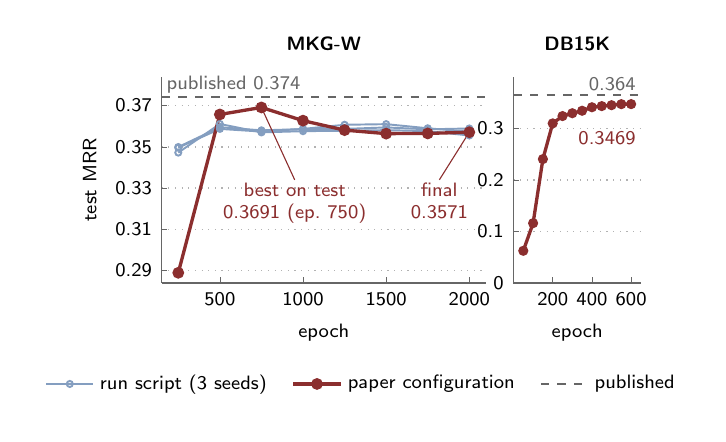
\begin{tikzpicture}
\begin{axis}[paperchart, name=mkgw, width=5.7cm, height=4.2cm, scale only axis=false,
  title={MKG-W}, xlabel={epoch}, ylabel={test MRR},
  xmin=150, xmax=2100, ymin=0.284, ymax=0.384, clip=false,
  xtick={500,1000,1500,2000}, ytick={0.29,0.31,0.33,0.35,0.37},
  yticklabel style={/pgf/number format/fixed, /pgf/number format/precision=2},
  xticklabel style={/pgf/number format/1000 sep={}},
  ymajorgrids, legend to name=curveslegend]
\addplot[nat!55, line width=0.7pt, mark=o, mark size=1.1pt] coordinates {(250,0.3496) (500,0.3587) (750,0.3574) (1000,0.3587) (1250,0.3607) (1500,0.3610) (1750,0.3590) (2000,0.3573)};
\addlegendentry{run script (3 seeds)}
\addplot[nat!55, line width=0.7pt, mark=o, mark size=1.1pt, forget plot] coordinates {(250,0.3472) (500,0.3611) (750,0.3570) (1000,0.3576) (1250,0.3578) (1500,0.3581) (1750,0.3576) (2000,0.3555)};
\addplot[nat!55, line width=0.7pt, mark=o, mark size=1.1pt, forget plot] coordinates {(250,0.3499) (500,0.3595) (750,0.3580) (1000,0.3586) (1250,0.3587) (1500,0.3594) (1750,0.3585) (2000,0.3589)};
\addplot[apk, line width=1.2pt, mark=*, mark size=1.5pt] coordinates {(250,0.2889) (500,0.3657) (750,0.3691) (1000,0.3627) (1250,0.3581) (1500,0.3564) (1750,0.3565) (2000,0.3571)};
\addlegendentry{paper configuration}
\addplot[black!60, dashed, line width=0.8pt, domain=150:2100, samples=2] {0.374};
\addlegendentry{published}
\draw[apk, line width=0.4pt] (axis cs:750,0.3691) -- (axis cs:950,0.334) node[font=\sffamily\scriptsize, anchor=north, inner sep=1pt, align=center] {best on test\\0.3691 (ep.\ 750)};
\draw[apk, line width=0.4pt] (axis cs:2000,0.3571) -- (axis cs:1820,0.334) node[font=\sffamily\scriptsize, anchor=north, inner sep=1pt, align=center] {final\\0.3571};
\node[font=\sffamily\scriptsize, text=black!60, anchor=south west, inner sep=1pt] at (axis cs:160,0.3745) {published 0.374};
\end{axis}
\begin{axis}[paperchart, at={(mkgw.east)}, anchor=west, xshift=0.35cm, width=3.2cm, height=4.2cm,
  title={DB15K}, xlabel={epoch},
  xmin=0, xmax=650, ymin=0, ymax=0.4, clip=false, xtick={200,400,600}, ytick={0,0.1,0.2,0.3},
  yticklabel style={/pgf/number format/fixed, /pgf/number format/precision=1}, ymajorgrids]
\addplot[apk, line width=1.2pt, mark=*, mark size=1.2pt] coordinates {(50,0.0623) (100,0.1159) (150,0.2402) (200,0.3095) (250,0.3237) (300,0.3292) (350,0.3340) (400,0.3408) (450,0.3430) (500,0.3448) (550,0.3468) (600,0.3469)};
\addplot[black!60, dashed, line width=0.8pt, domain=0:650, samples=2] {0.364};
\node[font=\sffamily\scriptsize, text=apk, anchor=north east, inner sep=1pt] at (axis cs:640,0.30) {0.3469};
\node[font=\sffamily\scriptsize, text=black!60, anchor=south east, inner sep=1pt] at (axis cs:640,0.367) {0.364};
\end{axis}
\node[anchor=north] at ([yshift=-0.9cm]$(mkgw.south west)!0.62!(mkgw.south east)$) {\pgfplotslegendfromname{curveslegend}};
\end{tikzpicture}
}
\caption{Test MRR during training (released code, our runs). The released code reports the highest point of each curve. W\&B: DB15K \wb{apkgc-repro/runs/y41uo30v}{y41uo30v}; MKG-W as in Table~\ref{tab:repro}.}
\label{fig:curves}
\end{figure}

The learning curves expose the effect of selecting on the test set. With the paper's
configuration MRR peaks at epoch 750 (0.3691) and declines to 0.3571 at epoch 2000; with
the run script the three seeds stay within 0.355-0.361 after epoch 500. Taking the last
epoch instead would lower the reported MRR by about 0.012 and 0.003 respectively.

This matters for the ranking claim, because NativE's released code reports its
\emph{final} checkpoint. We retrained NativE with its authors' MKG-W script (dimension 250,
batch 1024, 128 negatives, 1000 epochs) on the same feature files that APKGC uses, with
seeds 42 and 1234, and compare both models under both rules in Table~\ref{tab:native}.
With the final checkpoint, both NativE runs beat every APKGC run, by 0.0095 to 0.018 MRR;
with the best checkpoint on test the gap narrows but keeps its sign (0.3691 against 0.3730
and 0.3733). In our runs the paper's ranking is reversed. NativE has two seeds and each
model uses its own authors' configuration; selecting on the validation split would be the
proper protocol for both.

\begin{table}[!t]
\centering
\caption{APKGC and NativE on MKG-W under two checkpoint-selection rules (MRR, our runs, same feature files). W\&B: NativE \wb{apkgc-repro/runs/6vkgophb}{6vkgophb}, \wb{apkgc-repro/runs/e1ho9crp}{e1ho9crp}.}
\label{tab:native}
\small
\setlength{\tabcolsep}{3pt}
\begin{tabular}{lcc}
\toprule
 & final ckpt & best on test\\
\midrule
APKGC, run script, 3 seeds & 0.3572 $\pm$ 0.0017 & 0.3605 $\pm$ 0.0009\\
APKGC, paper config. & 0.3571 & 0.3691\\
NativE, seed 42 & 0.3684 & 0.3730\\
NativE, seed 1234 & 0.3733 & 0.3733\\
\midrule
Published~\cite{apkgc} & \multicolumn{2}{c}{APKGC 0.374, NativE 0.366}\\
\bottomrule
\end{tabular}
\end{table}

\subsection{The attention penalty}
\label{sec:c2}
The paper's ablation attributes 0.014 MRR to the penalty, and its own hyperparameter study
(Fig.~\ref{fig:heat}) already shows a weaker picture: on DB15K, 5 of the 16 penalised
configurations score below the $k=0$ row (0.340), which is constant in $\theta_p$ and
which we read as no penalty, and on MKG-W 8 of 16 score below it (one ties; Appendix~C). To test the claim we kept everything fixed
(MKG-W, seed 42, noise on, the released configuration and early stopping) and implemented
the penalty in four ways: \textbf{A}, the released code; \textbf{B}, exactly
Eqs.~(9)-(10); \textbf{C}, an adaptive criterion we propose, which penalises the most
probable token in the 10\% of rows with the lowest normalised attention entropy in each
batch, so no threshold needs tuning; and \textbf{B2}, clipping attention probabilities at
0.5 and spreading the excess to neighbours as in the paper's case study, the strongest
penalty.

\begin{figure}[!t]
\centering
% Figure: MRR on DB15K by window k and penalty rate theta_p (Section IV-B).
% Message: 5 of the 16 penalised configurations score below no penalty (k = 0, 0.340).
% source: the APKGC paper, hyperparameter study RQ4 (published numbers, redrawn).
% Cells below the no-penalty value are outlined.
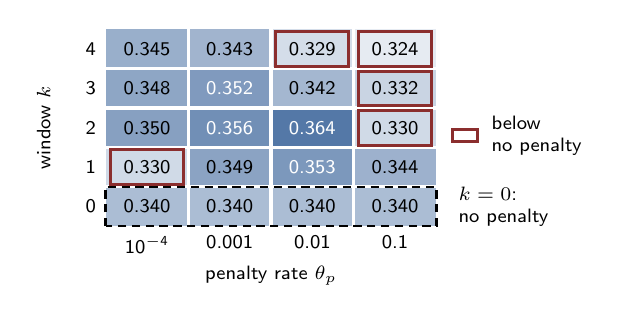
\begin{tikzpicture}[x=1.05cm, y=0.5cm, font=\sffamily\scriptsize]
\foreach \r/\a/\b/\c/\d in {4/0.345/0.343/0.329/0.324, 3/0.348/0.352/0.342/0.332, 2/0.350/0.356/0.364/0.330, 1/0.330/0.349/0.353/0.344, 0/0.340/0.340/0.340/0.340} {
  \foreach \v [count=\cc from 0] in {\a,\b,\c,\d} {
    \pgfmathsetmacro{\pc}{max(8,min(78,(\v-0.322)/0.043*70+8))}
    \fill[db!\pc] (\cc,\r) rectangle (\cc+1,\r+1);
    \pgfmathparse{\pc>55?"white":"black"}\edef\tc{\pgfmathresult}
    \node[text=\tc] at (\cc+0.5,\r+0.5) {\v};
  }
  \node[left] at (0,\r+0.5) {\r};
}
% cell borders drawn per line: `grid` steps in absolute cm, not in the picture's x/y units
\foreach \c in {1,2,3} \draw[white, line width=1.2pt] (\c,0) -- (\c,5);
\foreach \r in {1,2,3,4} \draw[white, line width=1.2pt] (0,\r) -- (4,\r);
% outline the penalised cells that score below no penalty (k = 0, 0.340)
\foreach \cc/\r in {2/4, 3/4, 3/3, 3/2, 0/1} \draw[dr, line width=1.1pt] (\cc+0.06,\r+0.06) rectangle (\cc+0.94,\r+0.94);
\draw[black, line width=0.9pt, dash pattern=on 3pt off 2pt] (0,0) rectangle (4,1);
\foreach \l [count=\cc from 0] in {{10\textsuperscript{$-$4}},0.001,0.01,0.1} \node[below] at (\cc+0.5,0) {\l};
\node at (2,-1.25) {penalty rate $\theta_p$};
\node[rotate=90] at (-0.75,2.5) {window $k$};
\node[anchor=west, align=left, font=\sffamily\scriptsize] at (4.15,0.5) {$k=0$:\\no penalty};
\draw[dr, line width=1pt] (4.2,2.15) rectangle (4.5,2.45); \node[anchor=west, font=\sffamily\scriptsize, align=left] at (4.55,2.3) {below\\no penalty};
\end{tikzpicture}

\caption{MRR on DB15K by window $k$ and penalty rate $\theta_p$, from the paper's hyperparameter study (RQ4)~\cite{apkgc}, redrawn. Dashed frame: $k=0$, constant in $\theta_p$, which we read as no penalty; red outline: penalised configurations that score below it. The paper's MKG-W panel (H@10) has 8 such cells out of 16.}
\label{fig:heat}
\end{figure}

\begin{table}[!t]
\centering
\caption{Four implementations of the attention penalty (MKG-W, seed 42). W\&B: A \wb{apkgc-repro/runs/5mubzabz}{5mubzabz}, B \wb{apkgc-repro/runs/n1z4asjp}{n1z4asjp}, C \wb{apkgc-repro/runs/5f540xf2}{5f540xf2}, B2 \wb{apkgc-repro/runs/6o5rs8sj}{6o5rs8sj}; firing counter \wb{apkgc-repro/runs/474c5kcn}{474c5kcn}.}
\label{tab:penalty}
\small
\begin{tabular}{llcc}
\toprule
 & Implementation & MRR & H@1\\
\midrule
A & released code & 0.3629 & 0.2933\\
B & Eqs.\ (9)-(10) & 0.3629 & 0.2933\\
C & entropy criterion (ours) & 0.3630 & 0.2934\\
B2 & clip at 0.5 & 0.3605 & 0.2964\\
\bottomrule
\end{tabular}
\end{table}

\begin{figure}[!t]
\centering
\resizebox{\columnwidth}{!}{% Figure: why the released attention penalty never fires (Section IV-B).
% Message: the paper compares each token's own score with phi; the released code compares the
% product of the scores from a position to the end of the row with 10. With scores of mean
% largest |A| per pass 7.50 on average (max 10.80) and 62.7% of suffix products negative, the condition
% held in 0 of 300 passes.
% source: experiments/results/apkgc_res/attn_scale.json (300 forward passes, firing counter);
% upstream/APKGC/mmkgc/module/model/APKGC.py (penalty condition). The word tokens are illustrative.
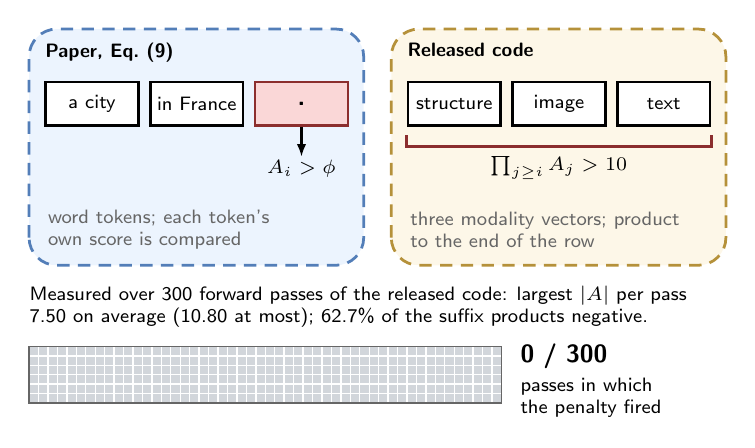
\begin{tikzpicture}[x=1cm, y=1cm, font=\sffamily\scriptsize,
  tok/.style={draw=black, line width=0.9pt, fill=white, minimum width=1.18cm, minimum height=0.55cm,
              inner sep=1pt, font=\sffamily\scriptsize},
  zone/.style={rounded corners=10pt, fill=#1!13, draw=#1!75!black, line width=1pt, dash pattern=on 4.5pt off 3pt},
  ztl/.style={font=\sffamily\scriptsize\bfseries, anchor=north west, inner sep=0pt},
  cond/.style={font=\sffamily\scriptsize, align=center, inner sep=1pt}]
% ---------- paper ----------
\draw[zone=bz] (0,0) rectangle (4.25,3.0);
\node[ztl] at (0.2,2.83) {Paper, Eq.~(9)};
\foreach \i/\n in {0/a city,1/in France,2/.}
  \node[tok] (p\i) at (0.8+1.33*\i,2.05) {\n};
\node[tok, fill=pk!45, draw=dr, font=\sffamily\small\bfseries] at (p2) {.};
\draw[-{Latex[length=1.6mm]}, line width=0.8pt] (p2.south) -- ++(0,-0.38);
\node[cond, anchor=north] at ([yshift=-0.38cm]p2.south) {$A_i>\phi$};
\node[cond, anchor=west, text=black!60, align=left] at (0.2,0.45) {word tokens; each token's\\own score is compared};
% ---------- released code ----------
\draw[zone=yz] (4.6,0) rectangle (8.85,3.0);
\node[ztl] at (4.8,2.83) {Released code};
\foreach \i/\n in {0/structure,1/image,2/text}
  \node[tok] (c\i) at (5.4+1.33*\i,2.05) {\n};
\draw[dr, line width=1pt] ([yshift=-3pt]c0.south west) -- ++(0,-0.15) -- ([yshift=-0.15cm-3pt]c2.south east) -- ++(0,0.15);
\node[cond, anchor=north] at ([yshift=-0.33cm]c1.south) {$\prod_{j\ge i} A_j>10$};
\node[cond, anchor=west, text=black!60, align=left] at (4.8,0.45) {three modality vectors; product\\to the end of the row};
% ---------- measured ----------
\node[font=\sffamily\scriptsize, anchor=north west, align=left, inner sep=0pt] at (0,-0.25)
  {Measured over 300 forward passes of the released code: largest $|A|$ per pass\\7.50 on average (10.80 at most); 62.7\% of the suffix products negative.};
% 300 passes as a 50 x 6 grid; none fired
\begin{scope}[shift={(0,-1.75)}]
\fill[gz!45] (0,0) rectangle (6.0,0.72);
\foreach \c in {1,...,49} \draw[white, line width=0.5pt] (0.12*\c,0) -- (0.12*\c,0.72);
\foreach \r in {1,...,5} \draw[white, line width=0.5pt] (0,0.12*\r) -- (6.0,0.12*\r);
\draw[black!60, line width=0.6pt] (0,0) rectangle (6.0,0.72);
\node[anchor=south west, font=\sffamily\small\bfseries, inner sep=1pt] at (6.2,0.4) {0 / 300};
\node[anchor=north west, font=\sffamily\scriptsize, align=left, inner sep=1pt] at (6.2,0.36) {passes in which\\the penalty fired};
\end{scope}
\end{tikzpicture}
}
\caption{Why the released penalty never fires. The paper compares each word token's score with $\phi$; the released code compares the product of the scores from a position to the end of a three-token row with 10. Grid: the 300 measured forward passes, none of which triggered the penalty. W\&B: \wb{apkgc-repro/runs/474c5kcn}{474c5kcn}.}
\label{fig:penalty}
\end{figure}

None of the four raises MRR (Table~\ref{tab:penalty}): A, B and C are at most 0.0001 apart,
nine times smaller than the std, and B2 is 0.0024 below A (2.7 std). To see why A and B
agree to four digits we attached a counter to the released code over 300 forward passes
(Fig.~\ref{fig:penalty}).
The released code compares the threshold 10 with the \emph{product} of the attention
scores from a position to the end of the row, not with the token's own score. The largest
absolute score in a pass is 7.50 on average (10.80 at most), and 62.7\% of the suffix
products are negative, so the condition is \textbf{never satisfied in any of the 300
passes}; the code then skips
the penalty block entirely. Variant A is in effect a model without the penalty, and B, with
$\theta_p=0.001$, removes only 0.1\% of the top token's score, which softmax barely
notices. A simulation that assumed independent scores had predicted a firing rate of
18-26\%; the measured 0\% shows that assumption is wrong on real data.

\emph{Are the penalised tokens the uninformative ones?} The paper supports this with two
case-study examples, not with a measurement over the dataset. In the released code the
question changes meaning, because the three tokens are whole modalities: a penalty, when it
fires, down-weights the structure, the image or the text of an entity, never a full stop.
Variant A penalises nothing and B almost nothing; C and B2 do penalise, but we did not log
which position, so whether they hit the right modality remains open. Logging the penalised
modality per query against the change in that query's rank would settle it cheaply.

\subsection{Adaptive noise sampling}
\label{sec:c3}
The paper describes $\theta_r$ as learned but does not report its value after training. We
read it from the best checkpoint of variant A, after checking the reading against known
constants in the same file ($\pi=3.14159$, margin $=12$). Table~\ref{tab:noise} shows that
$\theta_r$ falls from 0.7 to $-0.0004$, so the mix $(1-\theta_r)V_o+\theta_r N$ leaves the
original vector almost unchanged: the model switches the noise off by itself. This is what
one should expect when a noise level is optimised by the training loss, since corrupting
the input can only make that loss larger. $\theta_n$ stays at 0.2 because it receives no
gradient (Section~\ref{sec:flow}).

Consistently, a run with noise sampling switched off (no text, image or entity noise), otherwise
identical to A, gives MRR 0.3655, 0.0026 \emph{above} A. The difference is 2.96 std, just
below our 3-std rule, and comes from one seed with the Gaussian noise of the released code
rather than the uniform noise the paper states for MKG-W, so it does not settle the claim.
What it does show is that removing the noise does not lower MRR by 0.016 as the paper
reports.

\begin{table}[!t]
\centering
\caption{The noise component in the released code (MKG-W, seed 42). W\&B: parameters \wb{apkgc-repro/runs/xhepf56j}{xhepf56j}; without noise \wb{apkgc-repro/runs/2n68eify}{2n68eify}; with noise is variant A in Table~\ref{tab:penalty}.}
\label{tab:noise}
\small
\setlength{\tabcolsep}{4pt}
\begin{tabular}{lcc}
\toprule
 & initial & after training\\
\midrule
Mixing level $\theta_r$ & 0.7 & $-0.0004$\\
Sampling threshold $\theta_n$ & 0.2 & 0.2\\
\midrule
 & with noise & without noise\\
\midrule
MRR & 0.3629 & 0.3655\\
\bottomrule
\end{tabular}
\end{table}

\subsection{Robustness to corrupted modalities}
\label{sec:c4}
Robustness to noisy multi-modal data is the paper's first motivation, but the paper only
evaluates clean test data. We measured it directly. Without retraining, we corrupt the
frozen text and image features of all entities at test time in three kinds of ways (five
corruption types in all):
\emph{missing}, replacing a feature with the mean feature, which is how the released code
fills entities that lack a modality; \emph{swapped}, giving each entity another entity's
feature; and \emph{Gaussian} noise of $\sigma\in\{0.5,1,2\}$ times the per-dimension
standard deviation. Ranking follows the released filtered protocol exactly; as a check,
the uncorrupted condition reproduces each checkpoint's MRR to four digits. We evaluate
APKGC variant A (seeds 42 and 2024) and NativE (seeds 42 and 1234) with three random draws
per corruption; Fig.~\ref{fig:robust} shows the main conditions.

\begin{figure}[!t]
\centering
\resizebox{\columnwidth}{!}{% Figure: test-time corruption of MKG-W features, APKGC vs NativE (Section IV-D).
% Message: swapped text hurts far more than missing text, images barely matter, and APKGC is
% below NativE in every condition. Dumbbell per condition, grouped by corrupted modality.
% source: experiments/results/robustness/robustness_{apkgc_A_seed42,apkgc_A_seed2024,native_s42,
% native_s1234}.json, corruption rate 1.0, mean of the two training seeds per model
% (values checked by qa/verify_numbers.py).
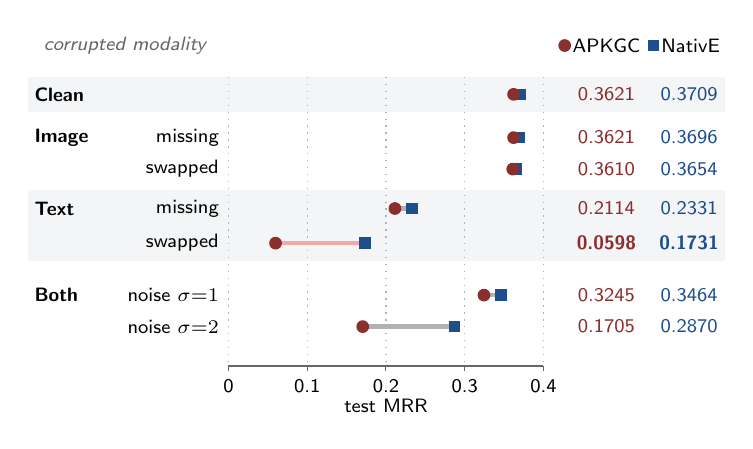
\begin{tikzpicture}[x=1cm, y=1cm, font=\sffamily\scriptsize,
  lbl/.style={font=\sffamily\scriptsize, anchor=east, inner sep=1pt},
  grp/.style={font=\sffamily\scriptsize\bfseries, anchor=west, inner sep=0pt},
  val/.style={font=\sffamily\scriptsize, inner sep=0pt},
  apkdot/.style={circle, fill=apk, inner sep=0pt, minimum size=4.6pt},
  natdot/.style={rectangle, fill=nat, inner sep=0pt, minimum size=4.2pt}]
\def\xo{2.55}\def\sc{10}          % plot origin (cm) and cm per unit MRR
% group bands
\foreach \t/\b in {0.22/-0.22, -1.22/-2.12} \fill[gz!11] (0,\t) rectangle (8.85,\b);
% dotted grid over the data rows only
\foreach \v in {0,0.1,0.2,0.3,0.4} \draw[black!30, dotted, line width=0.5pt] ({\xo+\sc*\v},0.22) -- ({\xo+\sc*\v},-3.45);
% rows: y / group / condition / APKGC / NativE / bold?
\foreach \y/\g/\c/\a/\n/\k in {
   0.00/Clean/{}/0.3621/0.3709/0,
  -0.55/Image/missing/0.3621/0.3696/0,
  -0.95/{}/swapped/0.3610/0.3654/0,
  -1.45/Text/missing/0.2114/0.2331/0,
  -1.89/{}/swapped/0.0598/0.1731/1,
  -2.55/{Both}/{noise $\sigma{=}1$}/0.3245/0.3464/0,
  -2.95/{}/{noise $\sigma{=}2$}/0.1705/0.2870/0} {
  \node[grp] at (0.08,\y) {\g};
  \node[lbl] at (\xo-0.08,\y) {\c};
  \ifnum\k=1 \def\lc{pk}\else\def\lc{black!30}\fi
  \draw[\lc, line width=1.6pt] ({\xo+\sc*\a},\y) -- ({\xo+\sc*\n},\y);
  \node[natdot] at ({\xo+\sc*\n},\y) {};
  \node[apkdot] at ({\xo+\sc*\a},\y) {};
  \ifnum\k=1
    \node[val, text=apk, font=\sffamily\scriptsize\bfseries] at (7.35,\y) {\a};
    \node[val, text=nat, font=\sffamily\scriptsize\bfseries] at (8.4,\y) {\n};
  \else
    \node[val, text=apk] at (7.35,\y) {\a};
    \node[val, text=nat] at (8.4,\y) {\n};
  \fi}
% column headers double as the legend
\node[apkdot] at (6.82,0.62) {}; \node[val] at (7.35,0.62) {APKGC};
\node[natdot] at (7.95,0.62) {}; \node[val] at (8.42,0.62) {NativE};
\node[font=\sffamily\scriptsize\itshape, anchor=west, text=black!60] at (0.08,0.62) {corrupted modality};
% x axis
\draw[black!60, line width=0.6pt] (\xo,-3.45) -- ({\xo+\sc*0.4},-3.45);
\foreach \v in {0,0.1,0.2,0.3,0.4} {
  \draw[black!60] ({\xo+\sc*\v},-3.45) -- ++(0,-0.06);
  \node[font=\sffamily\scriptsize, anchor=north] at ({\xo+\sc*\v},-3.5) {\v};}
\node[font=\sffamily\scriptsize] at ({\xo+\sc*0.2},-3.95) {test MRR};
\end{tikzpicture}
}
\caption{Test MRR on MKG-W when the text or image features of all entities are corrupted at test time; mean of two training seeds per model. W\&B: APKGC \wb{apkgc-repro/runs/pb3ucjeh}{pb3ucjeh}, \wb{apkgc-repro/runs/df5zub7c}{df5zub7c} (training of seed 2024: \wb{apkgc-repro/runs/lg894aew}{lg894aew}); NativE \wb{apkgc-repro/runs/o99pv1hz}{o99pv1hz}, \wb{apkgc-repro/runs/bv9nj30t}{bv9nj30t}.}
\label{fig:robust}
\end{figure}

Three findings stand out. \emph{Both models barely use images}: removing every image
changes APKGC's MRR by at most 0.0002 and NativE's by 0.0012 on average (0.0051 at most),
and swapping images costs at most 0.008, so on MKG-W the multi-modal model is in practice a
structure-plus-text model. \emph{Wrong text is far worse than no text}: with swapped text
APKGC falls to 0.0598, against 0.2114 when the text is simply absent. The model cannot tell
that a description belongs to another entity and follows it; this is over-trust at the
level of a whole modality, which the token-level penalty does not address. \emph{APKGC is
not more robust than NativE}: its MRR is lower in all 30 conditions we tested (five
corruption types, two corruption rates, three modality settings; Appendix~B), and its drop from the
clean value is larger in 17 of the 20 conditions that corrupt text; the three exceptions
are mild noise ($\sigma=0.5$), where the drops differ by at most 0.0015. NativE is not
APKGC without noise, so this does not isolate the noise component, but the paper's claim
predicts the opposite ordering, and the result agrees with $\theta_r$ being learned down
to 0.

\section{Discussion of APKGC}
The headline number of APKGC is approximately reproducible, but none of the paper's
explanations for it survives our tests. The evidence is strongest for the attention
penalty, which does not fire in the released code and gives no gain under four
implementations. For the noise, three independent observations point the same way: the
learned noise level goes to 0, removing noise does not hurt, and the model is less robust
than a baseline without this mechanism. The ranking over NativE does not hold once both
models are evaluated under one checkpoint-selection rule.

Reading the paper as a reviewer, we find further weaknesses that the reproduction alone
would not reveal.

\emph{Experimental protocol.} The headline numbers are the best cells of the paper's own
hyperparameter grid: 0.364 MRR on DB15K is the cell $k=2$, $\theta_p=0.01$, and 0.501 H@10
on MKG-W is the cell $k=1$, $\theta_p=0.01$. No validation split is described, so the
hyperparameters appear to be chosen on the test set, on top of the released code's
test-set checkpoint selection (Section~\ref{sec:c1}). There are no standard deviations,
numbers of runs, significance tests or training times; on DB15K the margin over NativE is
0.002 MRR and APKGC is lower on H@10 (0.527 against 0.529), which cannot be called an
improvement without variance estimates.

\emph{The penalty mechanism.} Eq.~(9) removes $\theta_p A^p_i$ from a token while Eq.~(10)
gives its neighbours $\theta^n_j(A^p_i-\phi)$, so attention mass is not conserved and
nothing renormalises it; the open window $(p-k,\,p+k)$ contains no neighbour when $k=1$;
and Eq.~(12) feeds the penalised attention scores to the encoder as if they were its input.
The equations do not say whether they act before or after softmax, although the case study
clips 0.66 and 0.59 to 0.5, which reads like probabilities. The motivation also transfers
poorly: OPERA~\cite{opera} describes over-trust during autoregressive decoding of
multi-modal language models, whereas APKGC applies it inside separate BERT and BEiT
encoders, where heavy attention on punctuation and separator tokens is known to act largely
as a no-op~\cite{clark}; in the paper's own case study the penalised tokens are ``for'' and
``and''. The hand-set $k=1$, $\theta_p=0.001$ in the released code is not the best grid cell
reported for either dataset.

\emph{The noise module.} The paper presents noise as a departure from methods that reject
it, yet its related work and RQ1 name SnAg and AdaMF as methods that already use noisy data;
the noise module is compared neither with them nor with plain regularisers such as dropout
or modality dropout. Eq.~(4) draws $U$ from $[\beta_{\min},\beta_{\max}]$ and then scales
it by $(\beta_{\max}-\beta_{\min})$ again, $\theta_n$ is ``adaptively tuned'' with no rule
given, and the choice of Gaussian noise for DB15K but uniform noise for MKG-W is neither
explained nor compared.

\emph{Ablations and claims.} The component ablation names no dataset; the modality ablation
covers DB15K only, and its structure-only variant (0.211 MRR) falls far below plain RotatE
(0.293), so its variants are not comparable baselines; and removing the attention
``decrease'' step costs only 0.005 MRR. RQ5 asks how APKGC performs on real-world data but
is answered with two hand-picked examples. Smaller inconsistencies: the experiments section
announces four research questions but lists five; the RQ1 text swaps the datasets of the
Hits@1 gains (the abstract has them right); H@3 on DB15K is 0.413 in the main table but
0.411 in the per-modality ablation; and the text omits $\phi$, $\theta^n_j$, the $\beta$
range, the initial $\theta_r$ and $\theta_n$, epochs, margin, optimiser and encoder
variants, so the method cannot be reproduced from the paper alone.

Our study has limits of its own: two seeds for NativE and for the robustness study, one
seed for the variant and ablation runs, Gaussian noise only, and checkpoints selected on
test, as in the released code. Settling the noise claim would take the no-noise variant on
seeds 1234, 2024 and 3407 under the protocol of Table~\ref{tab:repro}, the uniform noise of
Eq.~(4), and selection on the validation split for all models.

% ═══════════════════════════════ PART II ═══════════════════════════════
\section*{PART II: IMPARTAIL}

\section{Background and Method}
\subsection{Task and long-tail bias}
A scene graph has the triple structure of a knowledge graph, but subject and object are
objects in a video frame and the relation is their interaction, e.g.\ (person, holding,
cup). A spatio-temporal scene graph (STSG) assigns a graph to each frame and links the
graphs through object identities over time. ImparTail~\cite{impartail} addresses graph
generation for observed frames (VidSGG), which we reproduce, and anticipation for future
frames (SGA), as well as two robustness variants with 16 types of video corruption.
Evaluation has three modes, depending on what is given: PredCls (boxes and object labels;
only relations are predicted), SGCls (boxes) and SGDet (nothing); and three constraints:
\emph{with} (one relation per object pair in each group), \emph{no} (several allowed) and
\emph{semi} (several per pair, but only those scoring above a threshold, 0.9 in the
released code).

The benchmark, Action Genome~\cite{ag}, annotates person-object relations in Charades
videos~\cite{charades} with 26 predicates in three groups: attention (3), spatial (6) and
contacting (17). Counting the training annotations, there are 417,302 labelled
(person, object) pairs and the distribution is highly skewed: among the contacting
predicates, \emph{holding} appears 169,741 times and \emph{twisting} only 93 times, a ratio
of 1,825:1 (Fig.~\ref{fig:tail}).
A model trained for overall accuracy drifts towards common classes. Recall@$K$ (R@$K$),
computed over all predictions, hides this; mean Recall@$K$ (mR@$K$), the average of
per-class recall, exposes it.

\begin{figure}[!t]
\centering
\resizebox{\columnwidth}{!}{% Figure: long-tail distribution of the 17 contacting predicates in Action Genome (Section VI-A).
% Message: holding appears 169,741 times and twisting 93 times, a ratio of 1,825:1.
% source: experiments/results/impartail_repro/ag_predicate_freq.json (training annotations).
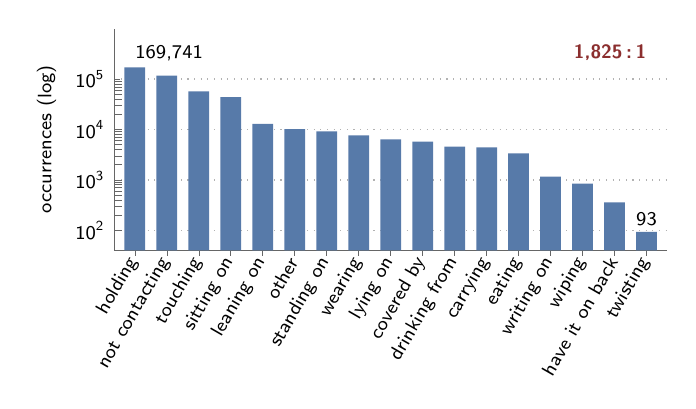
\begin{tikzpicture}
\begin{axis}[paperchart, width=8.6cm, height=4.4cm, ybar, bar width=7.5pt,
  ymode=log, log origin=infty, ymin=40, ymax=1e6, clip=false, ytick={1e2,1e3,1e4,1e5},
  yticklabels={{\sffamily 10\textsuperscript{2}},{\sffamily 10\textsuperscript{3}},{\sffamily 10\textsuperscript{4}},{\sffamily 10\textsuperscript{5}}},
  symbolic x coords={holding,not contacting,touching,sitting on,leaning on,other,standing on,wearing,lying on,covered by,drinking from,carrying,eating,writing on,wiping,have it on back,twisting},
  xtick=data, x tick label style={rotate=60, anchor=east, font=\sffamily\scriptsize, inner sep=1pt},
  ylabel={occurrences (log)}, enlarge x limits=0.04, ymajorgrids, axis x line*=bottom]
\addplot[fill=db!75, draw=none] coordinates {(holding,169741) (not contacting,117088) (touching,57033) (sitting on,43633) (leaning on,12944) (other,10084) (standing on,9124) (wearing,7611) (lying on,6330) (covered by,5705) (drinking from,4577) (carrying,4430) (eating,3355) (writing on,1159) (wiping,842) (have it on back,358) (twisting,93)};
\node[font=\sffamily\scriptsize, anchor=south west, inner sep=2pt, xshift=-2pt] at (axis cs:holding,169741) {169,741};
\node[font=\sffamily\scriptsize, anchor=south, inner sep=2pt] at (axis cs:twisting,93) {93};
\node[font=\sffamily\scriptsize\bfseries, text=dr, anchor=north east] at (rel axis cs:0.98,0.97) {1,825\,:\,1};
\end{axis}
\end{tikzpicture}
}
\caption{Occurrences of the 17 contacting predicates in the Action Genome training set (log scale), counted by us from the annotation file.}
\label{fig:tail}
\end{figure}

\subsection{Method}
ImparTail changes the objective, not the architecture (Fig.~\ref{fig:impartail}). Each
relation label $p^t_{ijk}$ (frame $t$, object pair $i,j$, predicate $k$) gets a binary mask
$m^t_{ijk}$, and the paper states that $m=1$ \emph{removes} the label from the loss:
\begin{equation}
\tilde{\mathcal{L}}_{p^t_{ijk}}=(1-m^t_{ijk})\,\mathcal{L}_{p^t_{ijk}}=\begin{cases}\mathcal{L}_{p^t_{ijk}} & m^t_{ijk}=0,\\ 0 & m^t_{ijk}=1.\end{cases} \tag{5}
\end{equation}
Algorithm~1 gives every predicate the same selection probability,
$\mathrm{Prob}[rel]=1/|P|$, and draws a per-predicate target count $\mathrm{Tar}[rel]$ from
a multinomial over $N_{\mathrm{target}}=N\times R_m$. The intent is that, because the count
is uniform over \emph{classes} rather than \emph{instances}, common classes lose more
labels and the learning signal shifts towards rare classes, without adding parameters. As
written, however, the appendix (Algorithm~2) \emph{masks} $\mathrm{Tar}[rel]$ instances of
each class: with $R_m=0.9$ that is about $0.9N/|P|$ per class, which would mask every
instance of any class rarer than that. The released code does the opposite, \emph{keeping}
$\mathrm{Tar}[rel]$ instances, drawn separately within each relation group; only this
reading matches the stated aim, and it is the one we analyse below. The paper also proposes raising the mask ratio with
the epoch ($R_m=e\times R_s$), but its Remark states that a fixed ratio of 0.9 performs
comparably and the reported numbers use it; the released code has no $R_m=e\times R_s$
schedule, only separate curriculum variants with a hard-coded one.

\begin{figure}[!t]
\centering
\resizebox{\columnwidth}{!}{% Figure: ImparTail as described in the paper (Section VI-B).
% Message: the baseline is unchanged; ImparTail only decides which labels enter the loss, so the
% gradient reaches the model only through unmasked labels. Schematic, no values.
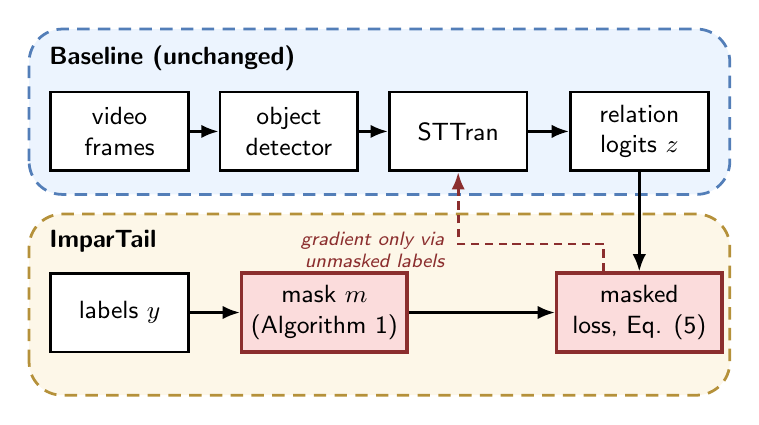
\begin{tikzpicture}[x=1cm, y=1cm, font=\sffamily\small,
  box/.style={draw=black, line width=1pt, fill=white, align=center, font=\sffamily\small, inner sep=2pt,
              minimum height=1cm, minimum width=1.75cm},
  ours/.style={box, fill=pk!40, draw=dr, line width=1.2pt},
  zone/.style={rounded corners=12pt, fill=#1!13, draw=#1!75!black, line width=1pt, dash pattern=on 4.5pt off 3pt},
  arr/.style={-{Latex[length=2.2mm, width=1.7mm]}, line width=1pt, draw=black},
  ztl/.style={font=\sffamily\small\bfseries, anchor=north west, inner sep=0pt}]
\draw[zone=bz] (-0.15,1.25) rectangle (8.75,3.35);
\draw[zone=yz] (-0.15,-1.3) rectangle (8.75,1.0);
\node[ztl] at (0.1,3.15) {Baseline (unchanged)};
\node[ztl] at (0.1,0.8) {ImparTail};
\node[box] (v) at (1.0,2.05) {video\\frames};
\node[box] (d) at (3.15,2.05) {object\\detector};
\node[box] (m) at (5.3,2.05) {STTran};
\node[box] (z) at (7.6,2.05) {relation\\logits $z$};
\node[box] (y) at (1.0,-0.25) {labels $y$};
\node[ours, minimum width=2.1cm] (a) at (3.6,-0.25) {mask $m$\\(Algorithm 1)};
\node[ours, minimum width=2.1cm] (L) at (7.6,-0.25) {masked\\loss, Eq. (5)};
\draw[arr] (v) -- (d); \draw[arr] (d) -- (m); \draw[arr] (m) -- (z);
\draw[arr] (z) -- (L); \draw[arr] (y) -- (a); \draw[arr] (a) -- (L);
\draw[-{Latex[length=2.2mm, width=1.7mm]}, line width=1pt, draw=dr, dash pattern=on 3pt off 2pt]
  ([xshift=-0.45cm]L.north) |- (5.3,0.62) -- (m.south);
\node[font=\sffamily\scriptsize\itshape, text=dr, anchor=east, align=right, inner sep=2pt] at (5.2,0.55) {gradient only via\\unmasked labels};
\end{tikzpicture}
}
\caption{ImparTail keeps the baseline architecture and changes only which labels enter the loss (red-bordered blocks). Drawn by us from the paper's description.}
\label{fig:impartail}
\end{figure}

\section{Experimental Setup}
For VidSGG the paper attaches ImparTail to STTran~\cite{sttran} and
DSG-DETR~\cite{dsgdetr}, trains both the baseline and ImparTail for five epochs with BCE
(the multi-label margin loss did not reproduce the literature's STTran numbers), and
reports mean Recall in its main table; for STTran in PredCls with the \emph{with}
constraint, mR@20 rises from 34.7 to 52.7, a relative gain of 51.9\% (18 points). Recall on
clean data appears only in the appendix, where the \emph{with}-constraint rows drop, e.g.\
R@50 of STTran in SGCls from 46.5 to 41.1.

We ran the authors' code on Kaggle (Tesla P100) in PredCls mode on all 1,750 Action Genome
test videos. Making it run required six environment fixes (a GPU-compatible build, outdated PyTorch and NumPy calls, and mounting the 58 GB of frame data), none of which changes the model. We use the
released STTran checkpoint for evaluation. For the mask experiment we train two variants
with the BCE loss, as the paper does, that differ only in the mask implementation: one run
each, two epochs, and no fixed seed, so the two runs also differ in their random mask draw
and initialisation.

\section{Results by Claim}
\subsection{Baseline reproduction}
\label{sec:i1}
Table~\ref{tab:it} compares nine mean Recall values of the released STTran checkpoint with
the paper: the mean deviation is 0.74 points and the largest 1.52 points. This validates
the evaluation pipeline, the data and the baseline checkpoint for mean Recall. Plain Recall
reproduces less well: under the \emph{with} constraint R@20 is 64.94 against the paper's
69.9.

\begin{table}[!t]
\centering
\caption{Mean Recall of STTran, PredCls: paper~\cite{impartail} $\to$ our evaluation of the released checkpoint. W\&B: \wb{impartail-repro/runs/emvvqpr2}{emvvqpr2}.}
\label{tab:it}
\small
\setlength{\tabcolsep}{4pt}
\begin{tabular}{lccc}
\toprule
Constraint & mR@10 & mR@20 & mR@50\\
\midrule
with & 30.5 $\to$ 30.70 & 34.7 $\to$ 35.54 & 34.8 $\to$ 35.65\\
no & 45.7 $\to$ 44.33 & 63.4 $\to$ 63.80 & 80.5 $\to$ 80.73\\
semi & 36.6 $\to$ 36.24 & 51.8 $\to$ 52.67 & 53.8 $\to$ 55.32\\
\bottomrule
\end{tabular}
\end{table}

The same evaluation reveals a property of the metric. Under the \emph{with} constraint,
R@20 is 64.94 and R@50 is 64.96. The evaluation code keeps one predicate per pair and
relation group, so a frame with at most 8 objects yields at most 24 candidates: R@50 equals
R@100 by construction, and R@20 can differ only on the few crowded frames (99.84\% of
training frames have at most 20 true labels, Fig.~\ref{fig:perframe}). Under \emph{semi} the
equality held empirically in our PredCls run. Large $K$ therefore adds little information
for comparing methods under these constraints.

\begin{figure}[!t]
\centering
\resizebox{\columnwidth}{!}{% Figure: relation labels per frame in Action Genome (Section VIII-A).
% Message: K = 20 already covers 99.84% of frames, so R@50 and R@100 cannot rise further under the
% with constraint.
% source: experiments/results/impartail_repro/ag_objects_per_frame.json ("nhan_moi_khung",
% training annotations, 198,973 frames).
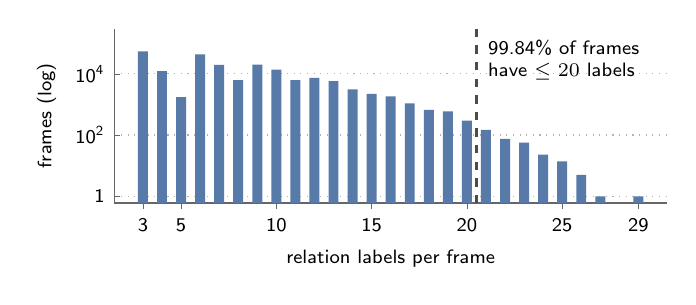
\begin{tikzpicture}
\begin{axis}[paperchart, width=8.6cm, height=3.8cm, ybar, bar width=3.6pt,
  ymode=log, log origin=infty, ymin=0.6, ymax=3e5, ytick={1,1e2,1e4},
  yticklabels={1,{\sffamily 10\textsuperscript{2}},{\sffamily 10\textsuperscript{4}}},
  xmin=1.5, xmax=30.5, xtick={3,5,10,15,20,25,29},
  xlabel={relation labels per frame}, ylabel={frames (log)}, ymajorgrids]
\addplot[fill=db!75, draw=none] coordinates {(3,53561) (4,12291) (5,1747) (6,43038) (7,19375) (8,6183) (9,19708) (10,13571) (11,6210) (12,7408) (13,5788) (14,3104) (15,2212) (16,1825) (17,1078) (18,664) (19,591) (20,295) (21,148) (22,75) (23,57) (24,23) (25,14) (26,5) (27,1) (29,1)};
\draw[black!70, dashed, line width=0.8pt] (axis cs:20.5,0.6) -- (axis cs:20.5,3e5);
\node[font=\sffamily\scriptsize, anchor=north west, align=left, inner sep=2pt] at (axis cs:20.8,2e5) {99.84\% of frames\\have $\le 20$ labels};
\end{axis}
\end{tikzpicture}
}
\caption{Relation labels per frame in the Action Genome training annotations (198,973 frames, log scale), counted by us.}
\label{fig:perframe}
\end{figure}

\subsection{The mask implementation}
\label{sec:i2}
With the binary cross-entropy (BCE) loss, the released code builds an all-zero target
vector, sets 1 only for labels that are \emph{not masked}, and averages BCE over the whole
vector; a pair whose labels in a group are all masked is skipped. A masked positive label
is therefore not removed from the loss as Eq.~(5) states whenever its pair keeps another
label of the same group: it becomes a \emph{negative label}. With a sigmoid, the gradient with respect to the logit
$z$ is $\partial\mathcal{L}/\partial z=q-y$, where $q$ is the predicted probability.
Fig.~\ref{fig:maskgrad} shows the three cases for a relation that is truly present: an
unmasked label pushes $q$ up, a label masked as in Eq.~(5) does nothing, and a label masked
as in the released code pushes $q$ \emph{down}.

\begin{figure}[!t]
\centering
\resizebox{\columnwidth}{!}{% Figure: what each mask treatment does to the predicted probability q of a relation that is
% truly present (Section VIII-B). BCE gradient w.r.t. the logit is q - y.
% Message: Eq. (5) removes a masked label (no push); the released code labels it 0 and pushes q
% down. The bar height q = 0.4 is illustrative; p_c = 0.016 for holding is from Algorithm 1 on
% Action Genome (experiments/tools/masked_bce_bias.py).
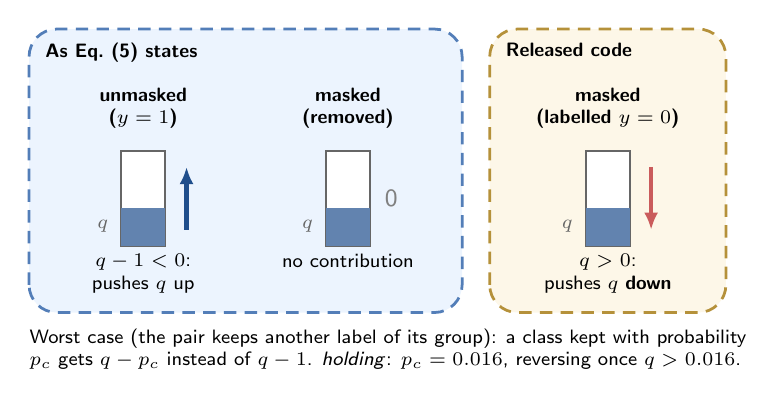
\begin{tikzpicture}[x=1cm, y=1cm, font=\sffamily\scriptsize,
  zone/.style={rounded corners=10pt, fill=#1!13, draw=#1!75!black, line width=1pt, dash pattern=on 4.5pt off 3pt},
  ztl/.style={font=\sffamily\scriptsize\bfseries, anchor=north west, inner sep=0pt},
  ttl/.style={font=\sffamily\scriptsize\bfseries, align=center, anchor=south, inner sep=1pt},
  note/.style={font=\sffamily\scriptsize, align=center, anchor=north, inner sep=1pt},
  push/.style={-{Latex[length=2.2mm, width=1.8mm]}, line width=1.6pt}]
\draw[zone=bz] (0,0) rectangle (5.5,3.6);
\node[ztl] at (0.2,3.43) {As Eq.~(5) states};
\draw[zone=yz] (5.85,0) rectangle (8.85,3.6);
\node[ztl] at (6.05,3.43) {Released code};
% one probability bar per case: x centre / title / arrow (1 up, 0 none, -1 down) / note
\foreach \x/\t/\d/\n in {1.45/{unmasked\\($y=1$)}/1/{$q-1<0$:\\pushes $q$ up},
                         4.05/{masked\\(removed)}/0/{no contribution},
                         7.35/{masked\\(labelled $y=0$)}/-1/{$q>0$:\\pushes $q$ \textbf{down}}} {
  \node[ttl] at (\x,2.3) {\t};
  \draw[black!60, line width=0.7pt, fill=white] (\x-0.28,0.85) rectangle (\x+0.28,2.05);
  \fill[db!70] (\x-0.28,0.85) rectangle (\x+0.28,1.33);
  \node[font=\sffamily\scriptsize, anchor=east, text=black!60] at (\x-0.32,1.09) {$q$};
  \ifnum\d=1 \draw[push, draw=db] (\x+0.55,1.05) -- (\x+0.55,1.85); \fi
  \ifnum\d=-1 \draw[push, draw=fail!90!black] (\x+0.55,1.85) -- (\x+0.55,1.05); \fi
  \ifnum\d=0 \node[font=\sffamily\small, text=black!50] at (\x+0.55,1.45) {0}; \fi
  \node[note] at (\x,0.78) {\n};}
% consequence for the most frequent class
\node[font=\sffamily\scriptsize, anchor=north west, align=left, inner sep=0pt] at (0,-0.2)
  {Worst case (the pair keeps another label of its group): a class kept with probability\\$p_c$ gets $q-p_c$ instead of $q-1$. \emph{holding}: $p_c=0.016$, reversing once $q>0.016$.};
\end{tikzpicture}
}
\caption{Effect of each mask treatment on the probability $q$ of a relation that is truly present (BCE gradient $q-y$; bar height illustrative).}
\label{fig:maskgrad}
\end{figure}

In the worst case, when the pair always keeps another label, a class kept with
probability $p_c$ receives the expected gradient $q-p_c$ instead of $q-1$, which reverses
once the model's confidence in a true relation exceeds $p_c$. Under the released code's
per-group sampling on Action Genome, \emph{holding} has $p_c=0.016$, while the four rarest
contacting classes have $p_c=1$ and are unaffected. The actual gradient lies between these
bounds because pairs with a single label in the group are skipped instead; the bias is
directional and largest on the common classes the method targets.

We patched the BCE loss to follow Eq.~(5), computing element-wise BCE, multiplying by
the mask and normalising by the number of active elements (which also rescales the loss),
and trained both variants. Table~\ref{tab:patch} shows that R@50 rises by 9.4 points under
\emph{with} and 11.4 points under \emph{semi}; the harmonic mean hR of R@50 and mR@50 rises
by 4.11 points on average over the three constraints. These differences must be read with
three caveats. First, the run-to-run noise is large: the attention predicates, whose loss is
identical in both variants, still move by up to 37 points (\emph{looking\_at} $+37.3$,
\emph{unsure} $-27.6$, Fig.~\ref{fig:perclass}), as much as \emph{holding} ($+42.2$) or
\emph{eating} ($-42.0$), so no per-class change can be attributed to the mask. Second, both
trained variants reach only 21.7 and 33.1 R@50 under \emph{semi}, against 83.27 for the
released checkpoint (Appendix~D): after two epochs most scores stay below the 0.9 threshold, so the
\emph{semi} gain reflects scores crossing that threshold more than better ranking. Third,
there is one unseeded run per variant, two epochs instead of the paper's five. The
experiment shows that the patch is feasible and points in a plausible direction; it does
not establish an improvement.

\begin{table}[!t]
\centering
\caption{Released mask $\to$ mask following Eq.~(5); STTran PredCls, one unseeded run per variant, two epochs. W\&B: released \wb{impartail-repro/runs/7ok1vx4f}{7ok1vx4f}, Eq.~(5) \wb{impartail-repro/runs/4h2scw2u}{4h2scw2u}.}
\label{tab:patch}
\small
\setlength{\tabcolsep}{3pt}
\begin{tabular}{lccc}
\toprule
Constraint & R@50 & mR@50 & $\Delta$hR@50\\
\midrule
with & 54.9 $\to$ 64.3 & 52.4 $\to$ 50.9 & $+3.2$\\
no & 99.6 $\to$ 99.6 & 97.6 $\to$ 96.5 & $-0.5$\\
semi & 21.7 $\to$ 33.1 & 13.8 $\to$ 22.2 & $+9.7$\\
\bottomrule
\end{tabular}
\end{table}

\begin{figure}[!t]
\centering
\resizebox{\columnwidth}{!}{% Figure: per-predicate change in R@50 (with constraint) from the released mask to Eq. (5)
% (Section VIII-B). Message: the largest gains are on frequent predicates, where the released
% mask biases the gradient most; several less frequent predicates lose recall. Attention predicates,
% untouched by the patch, move as much, so single-run per-class changes are within noise.
% Lollipop chart, predicates ordered by training frequency (most frequent on the left).
% source: experiments/results/impartail_repro/per_class_recall.json (va - goc, with, K=50)
% and ag_predicate_freq.json (training occurrences). One seed, two epochs.
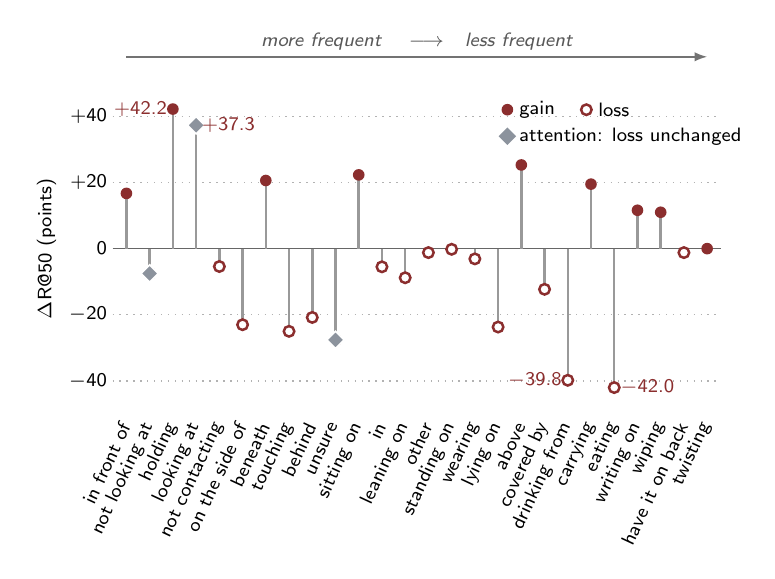
\begin{tikzpicture}[x=0.295cm, y=0.042cm, font=\sffamily\scriptsize]
% dotted grid over the data area only
\foreach \v in {-40,-20,20,40} \draw[black!30, dotted, line width=0.5pt] (-0.6,\v) -- (25.6,\v);
\draw[black!60, line width=0.6pt] (-0.6,0) -- (25.6,0);
\foreach \v/\t in {-40/$-$40,-20/$-$20,0/0,20/+20,40/+40} \node[anchor=east, inner sep=1pt] at (-0.7,\v) {\t};
\node[rotate=90, anchor=south] at (-2.6,0) {$\Delta$R@50 (points)};
% predicates: index / label / change
\foreach \i/\n/\d in {0/in front of/16.7, 1/not looking at/-7.5, 2/holding/42.2, 3/looking at/37.3,
  4/not contacting/-5.4, 5/on the side of/-23.0, 6/beneath/20.6, 7/touching/-25.0, 8/behind/-20.8,
  9/unsure/-27.6, 10/sitting on/22.3, 11/in/-5.5, 12/leaning on/-8.8, 13/other/-1.2,
  14/standing on/-0.2, 15/wearing/-3.1, 16/lying on/-23.7, 17/above/25.3, 18/covered by/-12.3,
  19/drinking from/-39.8, 20/carrying/19.5, 21/eating/-42.0, 22/writing on/11.6, 23/wiping/11.0,
  24/have it on back/-1.2, 25/twisting/0.0} {
  \draw[black!40, line width=0.9pt] (\i,0) -- (\i,\d);
  \pgfmathparse{\d>=0 ? 1 : 0}
  \ifnum\pgfmathresult=1
    \fill[dr] (\i,\d) circle (2.1pt);
  \else
    \draw[dr, fill=white, line width=0.9pt] (\i,\d) circle (1.9pt);
  \fi
  \node[rotate=65, anchor=east, inner sep=1pt] at (\i,-52) {\n};}
% attention predicates (indices 1, 3, 9): their CE loss is identical in both branches, so their
% change measures run-to-run noise; drawn as grey diamonds over the default marks
\foreach \i/\d in {1/-7.5, 3/37.3, 9/-27.6}
  \node[diamond, fill=gz!90!black, draw=white, line width=0.6pt, inner sep=0pt, minimum size=6.5pt] at (\i,\d) {};
% direct labels for the extremes named in the text
\foreach \i/\d/\t/\a in {2/42.2/+42.2/east, 3/37.3/+37.3/west, 19/-39.8/$-$39.8/east, 21/-42.0/$-$42.0/west}
  \node[anchor=\a, font=\sffamily\scriptsize, text=dr, inner sep=2pt] at (\i,\d) {\t};
% frequency direction
\draw[-{Latex[length=1.6mm]}, black!55, line width=0.6pt] (0,58) -- (25,58)
  node[pos=0.5, above, font=\sffamily\scriptsize\itshape, text=black!65, inner sep=2pt] {more frequent \quad$\longrightarrow$\quad less frequent};
% legend in one row below
\begin{scope}[shift={(16.4,42)}]
\fill[dr] (0,0) circle (2.1pt); \node[anchor=west, inner sep=2pt] at (0.25,0) {gain};
\draw[dr, fill=white, line width=0.9pt] (3.4,0) circle (1.9pt); \node[anchor=west, inner sep=2pt] at (3.65,0) {loss};
\node[diamond, fill=gz!90!black, inner sep=0pt, minimum size=6.5pt] at (0,-8) {}; \node[anchor=west, inner sep=2pt, align=left] at (0.25,-8) {attention: loss unchanged};
\end{scope}
\end{tikzpicture}
}
\caption{Per-predicate change in R@50 under the \emph{with} constraint from the released mask to Eq.~(5); predicates ordered by training frequency, filled dots are gains and open dots losses; grey diamonds are attention predicates, whose loss the patch does not change, so their spread shows the run-to-run noise (runs of Table~\ref{tab:patch}).}
\label{fig:perclass}
\end{figure}

\section{Discussion of ImparTail}
ImparTail is simple and general: it adds no parameters, attaches to several baselines and
raises mean Recall strongly in the paper's experiments. Our reproduction confirms the ground
those results stand on for mean Recall, the evaluation pipeline and the baseline
checkpoint, and finds that the released BCE mask turns masked labels into negatives instead
of removing them as Eq.~(5) states. Whether following the equation helps cannot be decided
from our single unseeded runs.

Reading the paper as a reviewer adds the following weaknesses. \emph{Trade-off.} The
Conclusion claims the gains come ``without sacrificing performance on head classes'', yet
clean-data Recall appears only in the appendix and drops in the \emph{with}-constraint rows;
the gains are reported as relative percentages (+51.9\% is 18 points), and no single number
such as hR summarises the trade-off. \emph{Baselines and statistics.} The method is close to
class-balanced undersampling, but it is not compared with simple long-tail remedies such as
inverse-frequency reweighting, class-balanced losses or logit adjustment; the baselines are
retrained in-house because the literature's STTran numbers did not reproduce; and no seeds,
standard deviations or significance tests are given, even for small differences. \emph{Protocol.} The released training code evaluates on the test split
every epoch and uses test R@20 to drive the learning-rate scheduler, and no validation
protocol is described. \emph{Specification.} Taken literally, the paper's mask algorithm
masks a fixed number of labels per class and would remove the rarest classes entirely;
only the released code's opposite reading rebalances classes as intended; the curriculum is described but not used for the reported numbers;
the \emph{semi} constraint depends on a score threshold the paper does not state; and the
robustness tasks apply image corruptions to methods that contain no robustness mechanism.
None of this negates the idea, but the size of the reported gains, and the claim that head
classes do not suffer, are not established by the evidence given.

% ═══════════════════════════════ CONCLUSION ═══════════════════════════════
\section{Conclusion}
Both papers' headline numbers can be approximately reproduced: APKGC reaches MRR 0.3691
against 0.374 on MKG-W with the paper's configuration, and ImparTail's STTran baseline is
within 0.74 mean Recall points on average (1.52 at most). The papers differ in what the numbers mean. For APKGC, the
attention penalty does not fire in the released code and gives no gain, the learned noise
level goes to 0, a retrained NativE beats APKGC under one shared protocol, and the
robustness that motivates the paper does not appear when measured. For ImparTail, the
released mask contradicts Eq.~(5), the written mask algorithm contradicts the method's own
aim, and whether following the equation helps cannot be decided from single unseeded runs
whose noise is as large as the effect. Across both, the most informative tests were not comparisons of final metrics
but direct measurements of intermediate quantities: how often a mechanism fires, what a
learned parameter converges to, and what the loss actually does to a masked label.

\section*{Appendix}
\subsection*{A. Per-seed results}
Table~\ref{tab:seeds} lists the three seeds behind the run-script row of
Table~\ref{tab:repro}.

\begin{table}[!h]
\centering
\caption{APKGC on MKG-W with the run-script configuration, per seed (best checkpoint on test). W\&B as in Table~\ref{tab:repro}.}
\label{tab:seeds}
\small
\setlength{\tabcolsep}{4pt}
\begin{tabular}{lccccc}
\toprule
Seed & MRR & H@1 & H@3 & H@10 & hours\\
\midrule
1234 & 0.3610 & 0.2987 & 0.3864 & 0.4759 & 3.2\\
2024 & 0.3611 & 0.2943 & 0.3907 & 0.4819 & 3.2\\
3407 & 0.3595 & 0.2925 & 0.3917 & 0.4799 & 3.2\\
\midrule
Mean & 0.3605 & 0.2952 & 0.3896 & 0.4792 & \\
\bottomrule
\end{tabular}
\end{table}

\subsection*{B. All 30 robustness conditions}
Table~\ref{tab:robustall} gives every condition of the study in Section~\ref{sec:c4}, of which
Fig.~\ref{fig:robust} shows seven. APKGC is lower than NativE in every cell.

\begin{table}[!h]
\centering
\caption{Test MRR on MKG-W under test-time corruption, APKGC / NativE (mean of two training seeds each; clean: 0.3621 / 0.3709). $p$: fraction of entities corrupted. W\&B as in Fig.~\ref{fig:robust}.}
\label{tab:robustall}
\scriptsize
\setlength{\tabcolsep}{2.5pt}
\begin{tabular}{llccc}
\toprule
Corruption & $p$ & image & text & both\\
\midrule
missing & 1.0 & 0.3621 / 0.3696 & 0.2114 / 0.2331 & 0.2096 / 0.2305\\
 & 0.5 & 0.3622 / 0.3707 & 0.2452 / 0.2810 & 0.2445 / 0.2816\\
swapped & 1.0 & 0.3610 / 0.3654 & 0.0598 / 0.1731 & 0.0589 / 0.1714\\
 & 0.5 & 0.3621 / 0.3680 & 0.1841 / 0.2568 & 0.1836 / 0.2567\\
noise $\sigma{=}0.5$ & 1.0 & 0.3619 / 0.3683 & 0.3554 / 0.3643 & 0.3549 / 0.3629\\
 & 0.5 & 0.3621 / 0.3694 & 0.3587 / 0.3669 & 0.3584 / 0.3657\\
noise $\sigma{=}1$ & 1.0 & 0.3578 / 0.3657 & 0.3294 / 0.3491 & 0.3245 / 0.3464\\
 & 0.5 & 0.3603 / 0.3678 & 0.3393 / 0.3550 & 0.3366 / 0.3524\\
noise $\sigma{=}2$ & 1.0 & 0.2911 / 0.3640 & 0.2292 / 0.2871 & 0.1705 / 0.2870\\
 & 0.5 & 0.3181 / 0.3671 & 0.2611 / 0.3109 & 0.2275 / 0.3092\\
\bottomrule
\end{tabular}
\end{table}

\subsection*{C. The paper's hyperparameter grid on MKG-W}
Fig.~\ref{fig:heatmkgw} redraws the MKG-W panel of the paper's RQ4 study, which reports
H@10 rather than MRR. The headline H@10 of 0.501 is the best cell, and 8 of the 16 penalised
configurations score below the $k=0$ row.

\begin{figure}[!h]
\centering
% Figure (appendix): H@10 on MKG-W by window k and penalty rate theta_p (Section IV-B).
% Message: 8 of the 16 penalised configurations score below the k = 0 row (0.491), one ties;
% the headline H@10 0.501 is the best cell (k = 1, theta_p = 0.01).
% source: the APKGC paper, hyperparameter study RQ4, Fig. 3(b) (published numbers, redrawn).
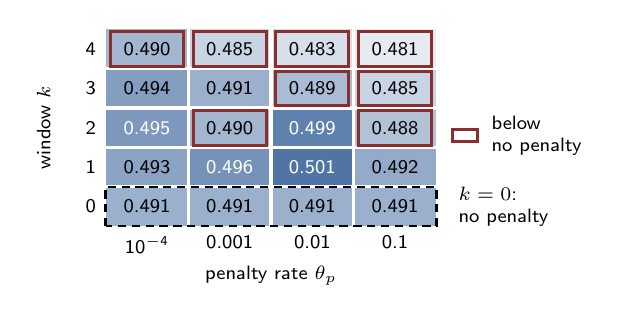
\begin{tikzpicture}[x=1.05cm, y=0.5cm, font=\sffamily\scriptsize]
\foreach \r/\a/\b/\c/\d in {4/0.490/0.485/0.483/0.481, 3/0.494/0.491/0.489/0.485, 2/0.495/0.490/0.499/0.488, 1/0.493/0.496/0.501/0.492, 0/0.491/0.491/0.491/0.491} {
  \foreach \v [count=\cc from 0] in {\a,\b,\c,\d} {
    \pgfmathsetmacro{\pc}{max(8,min(78,(\v-0.480)/0.021*70+8))}
    \fill[db!\pc] (\cc,\r) rectangle (\cc+1,\r+1);
    \pgfmathparse{\pc>55?"white":"black"}\edef\tc{\pgfmathresult}
    \node[text=\tc] at (\cc+0.5,\r+0.5) {\v};
  }
  \node[left] at (0,\r+0.5) {\r};
}
% cell borders drawn per line: `grid` steps in absolute cm, not in the picture's x/y units
\foreach \c in {1,2,3} \draw[white, line width=1.2pt] (\c,0) -- (\c,5);
\foreach \r in {1,2,3,4} \draw[white, line width=1.2pt] (0,\r) -- (4,\r);
% outline the penalised cells that score below the k = 0 row (0.491)
\foreach \cc/\r in {0/4, 1/4, 2/4, 3/4, 2/3, 3/3, 1/2, 3/2} \draw[dr, line width=1.1pt] (\cc+0.06,\r+0.06) rectangle (\cc+0.94,\r+0.94);
\draw[black, line width=0.9pt, dash pattern=on 3pt off 2pt] (0,0) rectangle (4,1);
\foreach \l [count=\cc from 0] in {{10\textsuperscript{$-$4}},0.001,0.01,0.1} \node[below] at (\cc+0.5,0) {\l};
\node at (2,-1.25) {penalty rate $\theta_p$};
\node[rotate=90] at (-0.75,2.5) {window $k$};
\node[anchor=west, align=left, font=\sffamily\scriptsize] at (4.15,0.5) {$k=0$:\\no penalty};
\draw[dr, line width=1pt] (4.2,2.15) rectangle (4.5,2.45); \node[anchor=west, font=\sffamily\scriptsize, align=left] at (4.55,2.3) {below\\no penalty};
\end{tikzpicture}

\caption{H@10 on MKG-W by window $k$ and penalty rate $\theta_p$, from the paper's hyperparameter study (RQ4)~\cite{apkgc}, redrawn. Red outline: penalised configurations below the $k=0$ row.}
\label{fig:heatmkgw}
\end{figure}

\subsection*{D. Full Recall of the ImparTail runs}
Table~\ref{tab:itall} gives Recall and mean Recall at three values of $K$ for the released
checkpoint and the two trained variants of Section~\ref{sec:i2}. Under \emph{semi}, both trained
variants give the same value at every $K$, a sign that few scores pass the 0.9 threshold
after two epochs.

\begin{table}[!h]
\centering
\caption{STTran PredCls: the released checkpoint (ckpt) and the two variants we trained, with the released mask (rel.) and following Eq.~(5). W\&B as in Tables~\ref{tab:it} and~\ref{tab:patch}.}
\label{tab:itall}
\scriptsize
\setlength{\tabcolsep}{2.4pt}
\begin{tabular}{llcccccc}
\toprule
 & & R@10 & R@20 & R@50 & mR@10 & mR@20 & mR@50\\
\midrule
with & ckpt & 62.0 & 64.9 & 65.0 & 30.7 & 35.5 & 35.6\\
 & rel. & 52.2 & 54.9 & 54.9 & 43.9 & 52.3 & 52.4\\
 & Eq.~5 & 61.1 & 64.3 & 64.3 & 42.8 & 50.7 & 50.9\\
\midrule
no & ckpt & 70.8 & 91.7 & 99.1 & 44.3 & 63.8 & 80.7\\
 & rel. & 70.0 & 90.3 & 99.6 & 56.7 & 77.0 & 97.6\\
 & Eq.~5 & 75.7 & 92.3 & 99.6 & 58.0 & 76.8 & 96.5\\
\midrule
semi & ckpt & 70.7 & 82.1 & 83.3 & 36.2 & 52.7 & 55.3\\
 & rel. & 21.7 & 21.7 & 21.7 & 13.8 & 13.8 & 13.8\\
 & Eq.~5 & 33.0 & 33.1 & 33.1 & 21.8 & 22.2 & 22.2\\
\bottomrule
\end{tabular}
\end{table}

\balance
\begin{thebibliography}{99}
\bibitem{apkgc} Y. Jian, X. Luo, Z. Li, M. Zhang, Y. Zhang, K. Xiao, and X. Hou, ``APKGC: Noise-enhanced multi-modal knowledge graph completion with attention penalty,'' in \emph{Proc. AAAI Conf. Artif. Intell.}, vol.~39, 2025, pp.~15005-15013.
\bibitem{impartail} R. Peddi, Saurabh, A. A. Shrivastava, P. Singla, and V. Gogate, ``Towards unbiased and robust spatio-temporal scene graph generation and anticipation,'' in \emph{Proc. IEEE/CVF Conf. Comput. Vis. Pattern Recognit. (CVPR)}, 2025.
\bibitem{ikrl} R. Xie, Z. Liu, H. Luan, and M. Sun, ``Image-embodied knowledge representation learning,'' in \emph{Proc. IJCAI}, 2017, pp.~3140-3146.
\bibitem{otkge} Z. Cao, Q. Xu, Z. Yang, Y. He, X. Cao, and Q. Huang, ``OTKGE: Multi-modal knowledge graph embeddings via optimal transport,'' in \emph{Proc. NeurIPS}, 2022.
\bibitem{native} Y. Zhang \emph{et al.}, ``NativE: Multi-modal knowledge graph completion in the wild,'' in \emph{Proc. 47th Int. ACM SIGIR Conf.}, 2024, pp.~91-101.
\bibitem{mkgw} D. Xu, T. Xu, S. Wu, J. Zhou, and E. Chen, ``Relation-enhanced negative sampling for multimodal knowledge graph completion,'' in \emph{Proc. 30th ACM Int. Conf. Multimedia}, 2022, pp.~3857-3866.
\bibitem{mans} Y. Zhang, M. Chen, and W. Zhang, ``Modality-aware negative sampling for multi-modal knowledge graph embedding,'' in \emph{Proc. IJCNN}, 2023.
\bibitem{adamf} Y. Zhang, Z. Chen, L. Liang, H. Chen, and W. Zhang, ``Unleashing the power of imbalanced modality information for multi-modal knowledge graph completion,'' in \emph{Proc. LREC-COLING}, 2024.
\bibitem{imf} X. Li, X. Zhao, J. Xu, Y. Zhang, and C. Xing, ``IMF: Interactive multimodal fusion model for link prediction,'' in \emph{Proc. ACM Web Conf. (WWW)}, 2023, pp.~2572-2580.
\bibitem{snag} Z. Chen \emph{et al.}, ``The power of noise: Toward a unified multi-modal knowledge graph representation framework,'' arXiv:2403.06832, 2024.
\bibitem{opera} Q. Huang \emph{et al.}, ``OPERA: Alleviating hallucination in multi-modal large language models via over-trust penalty and retrospection-allocation,'' arXiv:2311.17911, 2023.
\bibitem{bert} J. Devlin, M.-W. Chang, K. Lee, and K. Toutanova, ``BERT: Pre-training of deep bidirectional transformers for language understanding,'' in \emph{Proc. NAACL-HLT}, 2019, pp.~4171-4186.
\bibitem{beit} H. Bao, L. Dong, S. Piao, and F. Wei, ``BEiT: BERT pre-training of image transformers,'' in \emph{Proc. ICLR}, 2022.
\bibitem{rotate} Z. Sun, Z.-H. Deng, J.-Y. Nie, and J. Tang, ``RotatE: Knowledge graph embedding by relational rotation in complex space,'' in \emph{Proc. ICLR}, 2019.
\bibitem{apkgcrepo} HubuKG, ``APKGC,'' GitHub repository, 2025. [Online]. Available: \url{https://github.com/HubuKG/APKGC}
\bibitem{mmkg} Y. Liu, H. Li, A. García-Durán, M. Niepert, D. Oñoro-Rubio, and D. S. Rosenblum, ``MMKG: Multi-modal knowledge graphs,'' in \emph{Proc. ESWC}, 2019, pp.~459-474.
\bibitem{pairre} L. Chao, J. He, T. Wang, and W. Chu, ``PairRE: Knowledge graph embeddings via paired relation vectors,'' in \emph{Proc. ACL-IJCNLP}, 2021, pp.~4360-4369.
\bibitem{clark} K. Clark, U. Khandelwal, O. Levy, and C. D. Manning, ``What does BERT look at? An analysis of BERT's attention,'' in \emph{Proc. BlackboxNLP Workshop}, 2019, pp.~276-286.
\bibitem{ag} J. Ji, R. Krishna, L. Fei-Fei, and J. C. Niebles, ``Action Genome: Actions as compositions of spatio-temporal scene graphs,'' in \emph{Proc. CVPR}, 2020.
\bibitem{charades} G. A. Sigurdsson, G. Varol, X. Wang, A. Farhadi, I. Laptev, and A. Gupta, ``Hollywood in homes: Crowdsourcing data collection for activity understanding,'' in \emph{Proc. ECCV}, 2016.
\bibitem{sttran} Y. Cong, W. Liao, H. Ackermann, B. Rosenhahn, and M. Y. Yang, ``Spatial-temporal transformer for dynamic scene graph generation,'' in \emph{Proc. ICCV}, 2021.
\bibitem{dsgdetr} S. Feng, H. Mostafa, M. Nassar, S. Majumdar, and S. Tripathi, ``Exploiting long-term dependencies for generating dynamic scene graphs,'' in \emph{Proc. WACV}, 2023.
\end{thebibliography}

\end{document}
